
% Default to the notebook output style

    


% Inherit from the specified cell style.




    
\documentclass[11pt]{article}

    
    
    \usepackage[T1]{fontenc}
    % Nicer default font (+ math font) than Computer Modern for most use cases
    \usepackage{mathpazo}

    % Basic figure setup, for now with no caption control since it's done
    % automatically by Pandoc (which extracts ![](path) syntax from Markdown).
    \usepackage{graphicx}
    % We will generate all images so they have a width \maxwidth. This means
    % that they will get their normal width if they fit onto the page, but
    % are scaled down if they would overflow the margins.
    \makeatletter
    \def\maxwidth{\ifdim\Gin@nat@width>\linewidth\linewidth
    \else\Gin@nat@width\fi}
    \makeatother
    \let\Oldincludegraphics\includegraphics
    % Set max figure width to be 80% of text width, for now hardcoded.
    \renewcommand{\includegraphics}[1]{\Oldincludegraphics[width=.8\maxwidth]{#1}}
    % Ensure that by default, figures have no caption (until we provide a
    % proper Figure object with a Caption API and a way to capture that
    % in the conversion process - todo).
    \usepackage{caption}
    \DeclareCaptionLabelFormat{nolabel}{}
    \captionsetup{labelformat=nolabel}

    \usepackage{adjustbox} % Used to constrain images to a maximum size 
    \usepackage{xcolor} % Allow colors to be defined
    \usepackage{enumerate} % Needed for markdown enumerations to work
    \usepackage{geometry} % Used to adjust the document margins
    \usepackage{amsmath} % Equations
    \usepackage{amssymb} % Equations
    \usepackage{textcomp} % defines textquotesingle
    % Hack from http://tex.stackexchange.com/a/47451/13684:
    \AtBeginDocument{%
        \def\PYZsq{\textquotesingle}% Upright quotes in Pygmentized code
    }
    \usepackage{upquote} % Upright quotes for verbatim code
    \usepackage{eurosym} % defines \euro
    \usepackage[mathletters]{ucs} % Extended unicode (utf-8) support
    \usepackage[utf8x]{inputenc} % Allow utf-8 characters in the tex document
    \usepackage{fancyvrb} % verbatim replacement that allows latex
    \usepackage{grffile} % extends the file name processing of package graphics 
                         % to support a larger range 
    % The hyperref package gives us a pdf with properly built
    % internal navigation ('pdf bookmarks' for the table of contents,
    % internal cross-reference links, web links for URLs, etc.)
    \usepackage{hyperref}
    \usepackage{longtable} % longtable support required by pandoc >1.10
    \usepackage{booktabs}  % table support for pandoc > 1.12.2
    \usepackage[inline]{enumitem} % IRkernel/repr support (it uses the enumerate* environment)
    \usepackage[normalem]{ulem} % ulem is needed to support strikethroughs (\sout)
                                % normalem makes italics be italics, not underlines
    

    
    
    % Colors for the hyperref package
    \definecolor{urlcolor}{rgb}{0,.145,.698}
    \definecolor{linkcolor}{rgb}{.71,0.21,0.01}
    \definecolor{citecolor}{rgb}{.12,.54,.11}

    % ANSI colors
    \definecolor{ansi-black}{HTML}{3E424D}
    \definecolor{ansi-black-intense}{HTML}{282C36}
    \definecolor{ansi-red}{HTML}{E75C58}
    \definecolor{ansi-red-intense}{HTML}{B22B31}
    \definecolor{ansi-green}{HTML}{00A250}
    \definecolor{ansi-green-intense}{HTML}{007427}
    \definecolor{ansi-yellow}{HTML}{DDB62B}
    \definecolor{ansi-yellow-intense}{HTML}{B27D12}
    \definecolor{ansi-blue}{HTML}{208FFB}
    \definecolor{ansi-blue-intense}{HTML}{0065CA}
    \definecolor{ansi-magenta}{HTML}{D160C4}
    \definecolor{ansi-magenta-intense}{HTML}{A03196}
    \definecolor{ansi-cyan}{HTML}{60C6C8}
    \definecolor{ansi-cyan-intense}{HTML}{258F8F}
    \definecolor{ansi-white}{HTML}{C5C1B4}
    \definecolor{ansi-white-intense}{HTML}{A1A6B2}

    % commands and environments needed by pandoc snippets
    % extracted from the output of `pandoc -s`
    \providecommand{\tightlist}{%
      \setlength{\itemsep}{0pt}\setlength{\parskip}{0pt}}
    \DefineVerbatimEnvironment{Highlighting}{Verbatim}{commandchars=\\\{\}}
    % Add ',fontsize=\small' for more characters per line
    \newenvironment{Shaded}{}{}
    \newcommand{\KeywordTok}[1]{\textcolor[rgb]{0.00,0.44,0.13}{\textbf{{#1}}}}
    \newcommand{\DataTypeTok}[1]{\textcolor[rgb]{0.56,0.13,0.00}{{#1}}}
    \newcommand{\DecValTok}[1]{\textcolor[rgb]{0.25,0.63,0.44}{{#1}}}
    \newcommand{\BaseNTok}[1]{\textcolor[rgb]{0.25,0.63,0.44}{{#1}}}
    \newcommand{\FloatTok}[1]{\textcolor[rgb]{0.25,0.63,0.44}{{#1}}}
    \newcommand{\CharTok}[1]{\textcolor[rgb]{0.25,0.44,0.63}{{#1}}}
    \newcommand{\StringTok}[1]{\textcolor[rgb]{0.25,0.44,0.63}{{#1}}}
    \newcommand{\CommentTok}[1]{\textcolor[rgb]{0.38,0.63,0.69}{\textit{{#1}}}}
    \newcommand{\OtherTok}[1]{\textcolor[rgb]{0.00,0.44,0.13}{{#1}}}
    \newcommand{\AlertTok}[1]{\textcolor[rgb]{1.00,0.00,0.00}{\textbf{{#1}}}}
    \newcommand{\FunctionTok}[1]{\textcolor[rgb]{0.02,0.16,0.49}{{#1}}}
    \newcommand{\RegionMarkerTok}[1]{{#1}}
    \newcommand{\ErrorTok}[1]{\textcolor[rgb]{1.00,0.00,0.00}{\textbf{{#1}}}}
    \newcommand{\NormalTok}[1]{{#1}}
    
    % Additional commands for more recent versions of Pandoc
    \newcommand{\ConstantTok}[1]{\textcolor[rgb]{0.53,0.00,0.00}{{#1}}}
    \newcommand{\SpecialCharTok}[1]{\textcolor[rgb]{0.25,0.44,0.63}{{#1}}}
    \newcommand{\VerbatimStringTok}[1]{\textcolor[rgb]{0.25,0.44,0.63}{{#1}}}
    \newcommand{\SpecialStringTok}[1]{\textcolor[rgb]{0.73,0.40,0.53}{{#1}}}
    \newcommand{\ImportTok}[1]{{#1}}
    \newcommand{\DocumentationTok}[1]{\textcolor[rgb]{0.73,0.13,0.13}{\textit{{#1}}}}
    \newcommand{\AnnotationTok}[1]{\textcolor[rgb]{0.38,0.63,0.69}{\textbf{\textit{{#1}}}}}
    \newcommand{\CommentVarTok}[1]{\textcolor[rgb]{0.38,0.63,0.69}{\textbf{\textit{{#1}}}}}
    \newcommand{\VariableTok}[1]{\textcolor[rgb]{0.10,0.09,0.49}{{#1}}}
    \newcommand{\ControlFlowTok}[1]{\textcolor[rgb]{0.00,0.44,0.13}{\textbf{{#1}}}}
    \newcommand{\OperatorTok}[1]{\textcolor[rgb]{0.40,0.40,0.40}{{#1}}}
    \newcommand{\BuiltInTok}[1]{{#1}}
    \newcommand{\ExtensionTok}[1]{{#1}}
    \newcommand{\PreprocessorTok}[1]{\textcolor[rgb]{0.74,0.48,0.00}{{#1}}}
    \newcommand{\AttributeTok}[1]{\textcolor[rgb]{0.49,0.56,0.16}{{#1}}}
    \newcommand{\InformationTok}[1]{\textcolor[rgb]{0.38,0.63,0.69}{\textbf{\textit{{#1}}}}}
    \newcommand{\WarningTok}[1]{\textcolor[rgb]{0.38,0.63,0.69}{\textbf{\textit{{#1}}}}}
    
    
    % Define a nice break command that doesn't care if a line doesn't already
    % exist.
    \def\br{\hspace*{\fill} \\* }
    % Math Jax compatability definitions
    \def\gt{>}
    \def\lt{<}
    % Document parameters
    \title{TensorFlow-Introduction}
    
    
    

    % Pygments definitions
    
\makeatletter
\def\PY@reset{\let\PY@it=\relax \let\PY@bf=\relax%
    \let\PY@ul=\relax \let\PY@tc=\relax%
    \let\PY@bc=\relax \let\PY@ff=\relax}
\def\PY@tok#1{\csname PY@tok@#1\endcsname}
\def\PY@toks#1+{\ifx\relax#1\empty\else%
    \PY@tok{#1}\expandafter\PY@toks\fi}
\def\PY@do#1{\PY@bc{\PY@tc{\PY@ul{%
    \PY@it{\PY@bf{\PY@ff{#1}}}}}}}
\def\PY#1#2{\PY@reset\PY@toks#1+\relax+\PY@do{#2}}

\expandafter\def\csname PY@tok@w\endcsname{\def\PY@tc##1{\textcolor[rgb]{0.73,0.73,0.73}{##1}}}
\expandafter\def\csname PY@tok@c\endcsname{\let\PY@it=\textit\def\PY@tc##1{\textcolor[rgb]{0.25,0.50,0.50}{##1}}}
\expandafter\def\csname PY@tok@cp\endcsname{\def\PY@tc##1{\textcolor[rgb]{0.74,0.48,0.00}{##1}}}
\expandafter\def\csname PY@tok@k\endcsname{\let\PY@bf=\textbf\def\PY@tc##1{\textcolor[rgb]{0.00,0.50,0.00}{##1}}}
\expandafter\def\csname PY@tok@kp\endcsname{\def\PY@tc##1{\textcolor[rgb]{0.00,0.50,0.00}{##1}}}
\expandafter\def\csname PY@tok@kt\endcsname{\def\PY@tc##1{\textcolor[rgb]{0.69,0.00,0.25}{##1}}}
\expandafter\def\csname PY@tok@o\endcsname{\def\PY@tc##1{\textcolor[rgb]{0.40,0.40,0.40}{##1}}}
\expandafter\def\csname PY@tok@ow\endcsname{\let\PY@bf=\textbf\def\PY@tc##1{\textcolor[rgb]{0.67,0.13,1.00}{##1}}}
\expandafter\def\csname PY@tok@nb\endcsname{\def\PY@tc##1{\textcolor[rgb]{0.00,0.50,0.00}{##1}}}
\expandafter\def\csname PY@tok@nf\endcsname{\def\PY@tc##1{\textcolor[rgb]{0.00,0.00,1.00}{##1}}}
\expandafter\def\csname PY@tok@nc\endcsname{\let\PY@bf=\textbf\def\PY@tc##1{\textcolor[rgb]{0.00,0.00,1.00}{##1}}}
\expandafter\def\csname PY@tok@nn\endcsname{\let\PY@bf=\textbf\def\PY@tc##1{\textcolor[rgb]{0.00,0.00,1.00}{##1}}}
\expandafter\def\csname PY@tok@ne\endcsname{\let\PY@bf=\textbf\def\PY@tc##1{\textcolor[rgb]{0.82,0.25,0.23}{##1}}}
\expandafter\def\csname PY@tok@nv\endcsname{\def\PY@tc##1{\textcolor[rgb]{0.10,0.09,0.49}{##1}}}
\expandafter\def\csname PY@tok@no\endcsname{\def\PY@tc##1{\textcolor[rgb]{0.53,0.00,0.00}{##1}}}
\expandafter\def\csname PY@tok@nl\endcsname{\def\PY@tc##1{\textcolor[rgb]{0.63,0.63,0.00}{##1}}}
\expandafter\def\csname PY@tok@ni\endcsname{\let\PY@bf=\textbf\def\PY@tc##1{\textcolor[rgb]{0.60,0.60,0.60}{##1}}}
\expandafter\def\csname PY@tok@na\endcsname{\def\PY@tc##1{\textcolor[rgb]{0.49,0.56,0.16}{##1}}}
\expandafter\def\csname PY@tok@nt\endcsname{\let\PY@bf=\textbf\def\PY@tc##1{\textcolor[rgb]{0.00,0.50,0.00}{##1}}}
\expandafter\def\csname PY@tok@nd\endcsname{\def\PY@tc##1{\textcolor[rgb]{0.67,0.13,1.00}{##1}}}
\expandafter\def\csname PY@tok@s\endcsname{\def\PY@tc##1{\textcolor[rgb]{0.73,0.13,0.13}{##1}}}
\expandafter\def\csname PY@tok@sd\endcsname{\let\PY@it=\textit\def\PY@tc##1{\textcolor[rgb]{0.73,0.13,0.13}{##1}}}
\expandafter\def\csname PY@tok@si\endcsname{\let\PY@bf=\textbf\def\PY@tc##1{\textcolor[rgb]{0.73,0.40,0.53}{##1}}}
\expandafter\def\csname PY@tok@se\endcsname{\let\PY@bf=\textbf\def\PY@tc##1{\textcolor[rgb]{0.73,0.40,0.13}{##1}}}
\expandafter\def\csname PY@tok@sr\endcsname{\def\PY@tc##1{\textcolor[rgb]{0.73,0.40,0.53}{##1}}}
\expandafter\def\csname PY@tok@ss\endcsname{\def\PY@tc##1{\textcolor[rgb]{0.10,0.09,0.49}{##1}}}
\expandafter\def\csname PY@tok@sx\endcsname{\def\PY@tc##1{\textcolor[rgb]{0.00,0.50,0.00}{##1}}}
\expandafter\def\csname PY@tok@m\endcsname{\def\PY@tc##1{\textcolor[rgb]{0.40,0.40,0.40}{##1}}}
\expandafter\def\csname PY@tok@gh\endcsname{\let\PY@bf=\textbf\def\PY@tc##1{\textcolor[rgb]{0.00,0.00,0.50}{##1}}}
\expandafter\def\csname PY@tok@gu\endcsname{\let\PY@bf=\textbf\def\PY@tc##1{\textcolor[rgb]{0.50,0.00,0.50}{##1}}}
\expandafter\def\csname PY@tok@gd\endcsname{\def\PY@tc##1{\textcolor[rgb]{0.63,0.00,0.00}{##1}}}
\expandafter\def\csname PY@tok@gi\endcsname{\def\PY@tc##1{\textcolor[rgb]{0.00,0.63,0.00}{##1}}}
\expandafter\def\csname PY@tok@gr\endcsname{\def\PY@tc##1{\textcolor[rgb]{1.00,0.00,0.00}{##1}}}
\expandafter\def\csname PY@tok@ge\endcsname{\let\PY@it=\textit}
\expandafter\def\csname PY@tok@gs\endcsname{\let\PY@bf=\textbf}
\expandafter\def\csname PY@tok@gp\endcsname{\let\PY@bf=\textbf\def\PY@tc##1{\textcolor[rgb]{0.00,0.00,0.50}{##1}}}
\expandafter\def\csname PY@tok@go\endcsname{\def\PY@tc##1{\textcolor[rgb]{0.53,0.53,0.53}{##1}}}
\expandafter\def\csname PY@tok@gt\endcsname{\def\PY@tc##1{\textcolor[rgb]{0.00,0.27,0.87}{##1}}}
\expandafter\def\csname PY@tok@err\endcsname{\def\PY@bc##1{\setlength{\fboxsep}{0pt}\fcolorbox[rgb]{1.00,0.00,0.00}{1,1,1}{\strut ##1}}}
\expandafter\def\csname PY@tok@kc\endcsname{\let\PY@bf=\textbf\def\PY@tc##1{\textcolor[rgb]{0.00,0.50,0.00}{##1}}}
\expandafter\def\csname PY@tok@kd\endcsname{\let\PY@bf=\textbf\def\PY@tc##1{\textcolor[rgb]{0.00,0.50,0.00}{##1}}}
\expandafter\def\csname PY@tok@kn\endcsname{\let\PY@bf=\textbf\def\PY@tc##1{\textcolor[rgb]{0.00,0.50,0.00}{##1}}}
\expandafter\def\csname PY@tok@kr\endcsname{\let\PY@bf=\textbf\def\PY@tc##1{\textcolor[rgb]{0.00,0.50,0.00}{##1}}}
\expandafter\def\csname PY@tok@bp\endcsname{\def\PY@tc##1{\textcolor[rgb]{0.00,0.50,0.00}{##1}}}
\expandafter\def\csname PY@tok@fm\endcsname{\def\PY@tc##1{\textcolor[rgb]{0.00,0.00,1.00}{##1}}}
\expandafter\def\csname PY@tok@vc\endcsname{\def\PY@tc##1{\textcolor[rgb]{0.10,0.09,0.49}{##1}}}
\expandafter\def\csname PY@tok@vg\endcsname{\def\PY@tc##1{\textcolor[rgb]{0.10,0.09,0.49}{##1}}}
\expandafter\def\csname PY@tok@vi\endcsname{\def\PY@tc##1{\textcolor[rgb]{0.10,0.09,0.49}{##1}}}
\expandafter\def\csname PY@tok@vm\endcsname{\def\PY@tc##1{\textcolor[rgb]{0.10,0.09,0.49}{##1}}}
\expandafter\def\csname PY@tok@sa\endcsname{\def\PY@tc##1{\textcolor[rgb]{0.73,0.13,0.13}{##1}}}
\expandafter\def\csname PY@tok@sb\endcsname{\def\PY@tc##1{\textcolor[rgb]{0.73,0.13,0.13}{##1}}}
\expandafter\def\csname PY@tok@sc\endcsname{\def\PY@tc##1{\textcolor[rgb]{0.73,0.13,0.13}{##1}}}
\expandafter\def\csname PY@tok@dl\endcsname{\def\PY@tc##1{\textcolor[rgb]{0.73,0.13,0.13}{##1}}}
\expandafter\def\csname PY@tok@s2\endcsname{\def\PY@tc##1{\textcolor[rgb]{0.73,0.13,0.13}{##1}}}
\expandafter\def\csname PY@tok@sh\endcsname{\def\PY@tc##1{\textcolor[rgb]{0.73,0.13,0.13}{##1}}}
\expandafter\def\csname PY@tok@s1\endcsname{\def\PY@tc##1{\textcolor[rgb]{0.73,0.13,0.13}{##1}}}
\expandafter\def\csname PY@tok@mb\endcsname{\def\PY@tc##1{\textcolor[rgb]{0.40,0.40,0.40}{##1}}}
\expandafter\def\csname PY@tok@mf\endcsname{\def\PY@tc##1{\textcolor[rgb]{0.40,0.40,0.40}{##1}}}
\expandafter\def\csname PY@tok@mh\endcsname{\def\PY@tc##1{\textcolor[rgb]{0.40,0.40,0.40}{##1}}}
\expandafter\def\csname PY@tok@mi\endcsname{\def\PY@tc##1{\textcolor[rgb]{0.40,0.40,0.40}{##1}}}
\expandafter\def\csname PY@tok@il\endcsname{\def\PY@tc##1{\textcolor[rgb]{0.40,0.40,0.40}{##1}}}
\expandafter\def\csname PY@tok@mo\endcsname{\def\PY@tc##1{\textcolor[rgb]{0.40,0.40,0.40}{##1}}}
\expandafter\def\csname PY@tok@ch\endcsname{\let\PY@it=\textit\def\PY@tc##1{\textcolor[rgb]{0.25,0.50,0.50}{##1}}}
\expandafter\def\csname PY@tok@cm\endcsname{\let\PY@it=\textit\def\PY@tc##1{\textcolor[rgb]{0.25,0.50,0.50}{##1}}}
\expandafter\def\csname PY@tok@cpf\endcsname{\let\PY@it=\textit\def\PY@tc##1{\textcolor[rgb]{0.25,0.50,0.50}{##1}}}
\expandafter\def\csname PY@tok@c1\endcsname{\let\PY@it=\textit\def\PY@tc##1{\textcolor[rgb]{0.25,0.50,0.50}{##1}}}
\expandafter\def\csname PY@tok@cs\endcsname{\let\PY@it=\textit\def\PY@tc##1{\textcolor[rgb]{0.25,0.50,0.50}{##1}}}

\def\PYZbs{\char`\\}
\def\PYZus{\char`\_}
\def\PYZob{\char`\{}
\def\PYZcb{\char`\}}
\def\PYZca{\char`\^}
\def\PYZam{\char`\&}
\def\PYZlt{\char`\<}
\def\PYZgt{\char`\>}
\def\PYZsh{\char`\#}
\def\PYZpc{\char`\%}
\def\PYZdl{\char`\$}
\def\PYZhy{\char`\-}
\def\PYZsq{\char`\'}
\def\PYZdq{\char`\"}
\def\PYZti{\char`\~}
% for compatibility with earlier versions
\def\PYZat{@}
\def\PYZlb{[}
\def\PYZrb{]}
\makeatother


    % Exact colors from NB
    \definecolor{incolor}{rgb}{0.0, 0.0, 0.5}
    \definecolor{outcolor}{rgb}{0.545, 0.0, 0.0}



    
    % Prevent overflowing lines due to hard-to-break entities
    \sloppy 
    % Setup hyperref package
    \hypersetup{
      breaklinks=true,  % so long urls are correctly broken across lines
      colorlinks=true,
      urlcolor=urlcolor,
      linkcolor=linkcolor,
      citecolor=citecolor,
      }
    % Slightly bigger margins than the latex defaults
    
    \geometry{verbose,tmargin=1in,bmargin=1in,lmargin=1in,rmargin=1in}
    
    

    \begin{document}
    
    
    \maketitle
    
    

    
    \hypertarget{tensorflow-introduction}{%
\section{TensorFlow Introduction}\label{tensorflow-introduction}}

Dale Smith, Ph.D.~Math, Georgia Tech.

Data Scientist with FraudScope.

https://github.com/dtsmith2001

\hypertarget{preliminaries}{%
\subsection{Preliminaries}\label{preliminaries}}

I am using Anaconda 4.3.1. I ran

\begin{verbatim}
conda update --yes conda
conda update --all --yes
\end{verbatim}

TensorFlow can be installed via conda-forge but it's version 0.12. Use

\begin{verbatim}
pip install tensorflow
\end{verbatim}

For GPU use, follow the
\href{https://www.tensorflow.org/install/}{instructions}, or use an AWS
instance that is already configured. You can also build your own
instance; see
\url{http://expressionflow.com/2016/10/09/installing-tensorflow-on-an-aws-ec2-p2-gpu-instance/}
but note this uses an older version of TensorFlow.

I also installed
\href{https://github.com/transcranial/jupyter-themer}{jupyter-themer},
which is why my Pandas tables have every other row grey.

\hypertarget{tensorflow}{%
\subsection{TensorFlow}\label{tensorflow}}

TensorFlow was created internally at Google to serve as their AI
platform for deep learning, but it does more than deep learning or
neural networks. We will use it to train a linear regression model.

\href{https://keras.io}{Keras} was recently adopted by Google as their
neural network front-end. I highly recommend using Keras instead of
TensorFlow to build a neural network.

Many people believe Google open sourced TensorFlow because they realized
the data is more valuable than the code itself.

\hypertarget{declarative-versus-imperative-programming}{%
\subsection{Declarative versus Imperative
Programming}\label{declarative-versus-imperative-programming}}

With \textbf{declarative programming} you tell the computer what you
want to do, but not how to do it. This is what you do when you write an
SQL query or a program in TensorFlow.

\textbf{Imperative programming} requires you to tell the computer how to
do the job (Python, C/C++, C\#, etc).

\hypertarget{lets-get-started}{%
\subsection{Let's get started!}\label{lets-get-started}}

    \begin{Verbatim}[commandchars=\\\{\}]
{\color{incolor}In [{\color{incolor}1}]:} \PY{k+kn}{import} \PY{n+nn}{tensorflow} \PY{k}{as} \PY{n+nn}{tf}
        \PY{k+kn}{import} \PY{n+nn}{numpy} \PY{k}{as} \PY{n+nn}{np}
\end{Verbatim}


    \begin{Verbatim}[commandchars=\\\{\}]
{\color{incolor}In [{\color{incolor}2}]:} \PY{n}{hello} \PY{o}{=} \PY{n}{tf}\PY{o}{.}\PY{n}{constant}\PY{p}{(}\PY{l+s+s1}{\PYZsq{}}\PY{l+s+s1}{Hello, TensorFlow!}\PY{l+s+s1}{\PYZsq{}}\PY{p}{)}
        \PY{n}{hello}
\end{Verbatim}


\begin{Verbatim}[commandchars=\\\{\}]
{\color{outcolor}Out[{\color{outcolor}2}]:} <tf.Tensor 'Const:0' shape=() dtype=string>
\end{Verbatim}
            
    \begin{Verbatim}[commandchars=\\\{\}]
{\color{incolor}In [{\color{incolor}3}]:} \PY{n}{sess} \PY{o}{=} \PY{n}{tf}\PY{o}{.}\PY{n}{Session}\PY{p}{(}\PY{p}{)}
\end{Verbatim}


    \textbf{Note}: Nothing happens until you run the session.

    \begin{Verbatim}[commandchars=\\\{\}]
{\color{incolor}In [{\color{incolor}4}]:} \PY{n+nb}{print}\PY{p}{(}\PY{n}{sess}\PY{o}{.}\PY{n}{run}\PY{p}{(}\PY{n}{hello}\PY{p}{)}\PY{p}{)}
\end{Verbatim}


    \begin{Verbatim}[commandchars=\\\{\}]
b'Hello, TensorFlow!'

    \end{Verbatim}

    \hypertarget{computational-graphs}{%
\subsection{Computational Graphs}\label{computational-graphs}}

Yes, these are real graph structures. I would describe them as acyclic
directed graphs. These structures are often used to find best paths to
recompute, say, bond prices.

A \textbf{computational graph} is a series of operations (+, -, etc)
expressed as nodes of the graph. Each node takes a tensor as input and a
tensor as output.

A \textbf{\href{https://en.wikipedia.org/wiki/Tensor}{tensor}} is an
object represented as a multidimensional array with respect to a basis,
much as a matrix is a representation of a \textbf{linear transformation}
with respect to a basis. The Stress tensor and curvature tensor are used
extensively in elastic materials and general relativity. Tensors were
also used in psychology to handle multidimensional data, and more
recently in machine learning.

\hypertarget{create-nodes-and-visualize-a-simple-computation-graph}{%
\subsubsection{Create Nodes and Visualize a Simple Computation
Graph}\label{create-nodes-and-visualize-a-simple-computation-graph}}

We can create a constant node as

    \begin{Verbatim}[commandchars=\\\{\}]
{\color{incolor}In [{\color{incolor}5}]:} \PY{n}{node1} \PY{o}{=} \PY{n}{tf}\PY{o}{.}\PY{n}{constant}\PY{p}{(}\PY{l+m+mf}{3.0}\PY{p}{)}
\end{Verbatim}


    \begin{Verbatim}[commandchars=\\\{\}]
{\color{incolor}In [{\color{incolor}6}]:} \PY{n}{node2} \PY{o}{=} \PY{n}{tf}\PY{o}{.}\PY{n}{constant}\PY{p}{(}\PY{l+m+mf}{4.0}\PY{p}{)}
\end{Verbatim}


    \begin{Verbatim}[commandchars=\\\{\}]
{\color{incolor}In [{\color{incolor}7}]:} \PY{n}{node2}
\end{Verbatim}


\begin{Verbatim}[commandchars=\\\{\}]
{\color{outcolor}Out[{\color{outcolor}7}]:} <tf.Tensor 'Const\_2:0' shape=() dtype=float32>
\end{Verbatim}
            
    Add two objects:

    \begin{Verbatim}[commandchars=\\\{\}]
{\color{incolor}In [{\color{incolor}8}]:} \PY{n}{node3} \PY{o}{=} \PY{n}{tf}\PY{o}{.}\PY{n}{add}\PY{p}{(}\PY{n}{node1}\PY{p}{,} \PY{n}{node2}\PY{p}{)}
        \PY{n}{node3}
\end{Verbatim}


\begin{Verbatim}[commandchars=\\\{\}]
{\color{outcolor}Out[{\color{outcolor}8}]:} <tf.Tensor 'Add:0' shape=() dtype=float32>
\end{Verbatim}
            
    \begin{Verbatim}[commandchars=\\\{\}]
{\color{incolor}In [{\color{incolor}9}]:} \PY{n}{sess} \PY{o}{=} \PY{n}{tf}\PY{o}{.}\PY{n}{Session}\PY{p}{(}\PY{p}{)}
\end{Verbatim}


    \begin{Verbatim}[commandchars=\\\{\}]
{\color{incolor}In [{\color{incolor}10}]:} \PY{n+nb}{print}\PY{p}{(}\PY{l+s+s2}{\PYZdq{}}\PY{l+s+s2}{sess.run(node3): }\PY{l+s+s2}{\PYZdq{}}\PY{p}{,} \PY{n}{sess}\PY{o}{.}\PY{n}{run}\PY{p}{(}\PY{n}{node3}\PY{p}{)}\PY{p}{)}
\end{Verbatim}


    \begin{Verbatim}[commandchars=\\\{\}]
sess.run(node3):  7.0

    \end{Verbatim}

    \begin{Verbatim}[commandchars=\\\{\}]
{\color{incolor}In [{\color{incolor}11}]:} \PY{n}{node4} \PY{o}{=} \PY{n}{tf}\PY{o}{.}\PY{n}{constant}\PY{p}{(}\PY{l+m+mf}{10.0}\PY{p}{)}
\end{Verbatim}


    \begin{Verbatim}[commandchars=\\\{\}]
{\color{incolor}In [{\color{incolor}12}]:} \PY{n}{node5} \PY{o}{=} \PY{n}{tf}\PY{o}{.}\PY{n}{add}\PY{p}{(}\PY{n}{node3}\PY{p}{,} \PY{n}{node4}\PY{p}{)}
\end{Verbatim}


    TensorFlow comes with an application called \textbf{TensorBoard} which
we can use to visualize the computational graph for the nodes we've
constructed.

    \begin{Verbatim}[commandchars=\\\{\}]
{\color{incolor}In [{\color{incolor}13}]:} \PY{n}{graph} \PY{o}{=} \PY{n}{tf}\PY{o}{.}\PY{n}{get\PYZus{}default\PYZus{}graph}\PY{p}{(}\PY{p}{)}
         \PY{n}{summary\PYZus{}writer} \PY{o}{=} \PY{n}{tf}\PY{o}{.}\PY{n}{summary}\PY{o}{.}\PY{n}{FileWriter}\PY{p}{(}\PY{l+s+s2}{\PYZdq{}}\PY{l+s+s2}{/Users/driver.dan12/Temp}\PY{l+s+s2}{\PYZdq{}}\PY{p}{,} \PY{n}{graph}\PY{p}{)}
         \PY{n}{summary\PYZus{}writer}\PY{o}{.}\PY{n}{flush}\PY{p}{(}\PY{p}{)}
\end{Verbatim}


    Now run \texttt{tensorboard\ -\/-logdir=/Users/driver.dan12/Temp} and
click on http://localhost:6006. Here is the computation graph
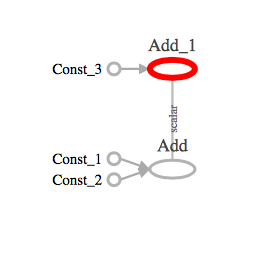
\includegraphics{graph1.png}.

    \hypertarget{warnings-from-tensorflow}{%
\subsection{Warnings from TensorFlow}\label{warnings-from-tensorflow}}

\begin{quote}
\texttt{The\ TensorFlow\ library\ wasn\textquotesingle{}t\ compiled\ to\ use\ SSE4.1\ instructions,\ but\ these\ are\ available\ on\ your\ machine\ and\ could\ speed\ up\ CPU\ computations.}
\end{quote}

Compile your own TensorFlow. See
http://stackoverflow.com/questions/42270739/how-do-i-resolve-these-tensorflow-warnings/42975902\#42975902.

    Let's clear the default graph and take a look at this more closely.

    \begin{Verbatim}[commandchars=\\\{\}]
{\color{incolor}In [{\color{incolor}14}]:} \PY{n}{tf}\PY{o}{.}\PY{n}{reset\PYZus{}default\PYZus{}graph}\PY{p}{(}\PY{p}{)}
\end{Verbatim}


    \hypertarget{does-this-look-odd}{%
\subsection{Does this look odd?}\label{does-this-look-odd}}

    \begin{Verbatim}[commandchars=\\\{\}]
{\color{incolor}In [{\color{incolor}15}]:} \PY{n}{x} \PY{o}{=} \PY{n}{tf}\PY{o}{.}\PY{n}{Variable}\PY{p}{(}\PY{l+m+mi}{0}\PY{p}{,} \PY{n}{name}\PY{o}{=}\PY{l+s+s1}{\PYZsq{}}\PY{l+s+s1}{x}\PY{l+s+s1}{\PYZsq{}}\PY{p}{)}
         \PY{n}{model} \PY{o}{=} \PY{n}{tf}\PY{o}{.}\PY{n}{global\PYZus{}variables\PYZus{}initializer}\PY{p}{(}\PY{p}{)}
         \PY{k}{with} \PY{n}{tf}\PY{o}{.}\PY{n}{Session}\PY{p}{(}\PY{p}{)} \PY{k}{as} \PY{n}{session}\PY{p}{:}
             \PY{k}{for} \PY{n}{i} \PY{o+ow}{in} \PY{n+nb}{range}\PY{p}{(}\PY{l+m+mi}{5}\PY{p}{)}\PY{p}{:}
                 \PY{n}{session}\PY{o}{.}\PY{n}{run}\PY{p}{(}\PY{n}{model}\PY{p}{)}
                 \PY{n}{x} \PY{o}{=} \PY{n}{x} \PY{o}{+} \PY{l+m+mi}{1}
                 \PY{n+nb}{print}\PY{p}{(}\PY{n}{session}\PY{o}{.}\PY{n}{run}\PY{p}{(}\PY{n}{x}\PY{p}{)}\PY{p}{)}
\end{Verbatim}


    \begin{Verbatim}[commandchars=\\\{\}]
1
2
3
4
5

    \end{Verbatim}

    \begin{Verbatim}[commandchars=\\\{\}]
{\color{incolor}In [{\color{incolor}16}]:} \PY{n}{x} \PY{o}{=} \PY{n}{tf}\PY{o}{.}\PY{n}{Variable}\PY{p}{(}\PY{l+m+mi}{0}\PY{p}{,} \PY{n}{name}\PY{o}{=}\PY{l+s+s1}{\PYZsq{}}\PY{l+s+s1}{x}\PY{l+s+s1}{\PYZsq{}}\PY{p}{)}
         \PY{n}{model} \PY{o}{=} \PY{n}{tf}\PY{o}{.}\PY{n}{global\PYZus{}variables\PYZus{}initializer}\PY{p}{(}\PY{p}{)}
         \PY{k}{with} \PY{n}{tf}\PY{o}{.}\PY{n}{Session}\PY{p}{(}\PY{p}{)} \PY{k}{as} \PY{n}{session}\PY{p}{:}
             \PY{k}{for} \PY{n}{i} \PY{o+ow}{in} \PY{n+nb}{range}\PY{p}{(}\PY{l+m+mi}{5}\PY{p}{)}\PY{p}{:}
                 \PY{n}{x} \PY{o}{=} \PY{n}{x} \PY{o}{+} \PY{l+m+mi}{1}
                 \PY{n}{session}\PY{o}{.}\PY{n}{run}\PY{p}{(}\PY{n}{model}\PY{p}{)}
                 \PY{n+nb}{print}\PY{p}{(}\PY{n}{session}\PY{o}{.}\PY{n}{run}\PY{p}{(}\PY{n}{x}\PY{p}{)}\PY{p}{)}
\end{Verbatim}


    \begin{Verbatim}[commandchars=\\\{\}]
1
2
3
4
5

    \end{Verbatim}

    Nope, this makes perfect sense - we are not executing the computation
graph until the \texttt{run} command. So whether we put the
\texttt{x\ =\ x\ +\ 1} before or after \texttt{session.run(model)}. This
statement initializes \texttt{x} to be zero, and \texttt{run} executes
the computation graph built so far.

But what does \texttt{global\_variables\_initializer} do?

It initializes all the \emph{global variables} in the graph. The global
variables are shared across machines in a distributed environment.
Contrast with \emph{local variables} which are per-process variables.

We don't need to initialize \texttt{Constant}, just \texttt{Variable}.
Reflect on that a little bit.

    \begin{Verbatim}[commandchars=\\\{\}]
{\color{incolor}In [{\color{incolor}17}]:} \PY{n}{graph} \PY{o}{=} \PY{n}{tf}\PY{o}{.}\PY{n}{get\PYZus{}default\PYZus{}graph}\PY{p}{(}\PY{p}{)}
         \PY{n}{summary\PYZus{}writer} \PY{o}{=} \PY{n}{tf}\PY{o}{.}\PY{n}{summary}\PY{o}{.}\PY{n}{FileWriter}\PY{p}{(}\PY{l+s+s2}{\PYZdq{}}\PY{l+s+s2}{/Users/driver.dan12/Temp}\PY{l+s+s2}{\PYZdq{}}\PY{p}{,} \PY{n}{graph}\PY{p}{)}
         \PY{n}{summary\PYZus{}writer}\PY{o}{.}\PY{n}{flush}\PY{p}{(}\PY{p}{)}
\end{Verbatim}


    Here is the computation graph 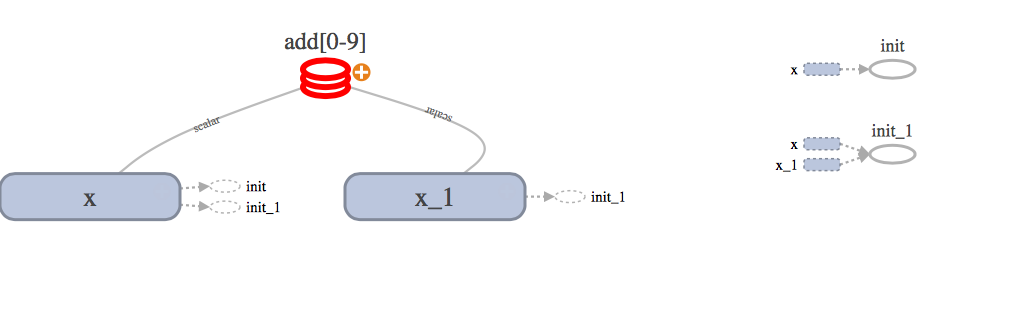
\includegraphics{graph2.png}

    \begin{Verbatim}[commandchars=\\\{\}]
{\color{incolor}In [{\color{incolor}18}]:} \PY{n}{tf}\PY{o}{.}\PY{n}{reset\PYZus{}default\PYZus{}graph}\PY{p}{(}\PY{p}{)}
\end{Verbatim}


    \hypertarget{matrix-multiplication}{%
\subsection{Matrix Multiplication}\label{matrix-multiplication}}

    \begin{Verbatim}[commandchars=\\\{\}]
{\color{incolor}In [{\color{incolor}19}]:} \PY{n}{W} \PY{o}{=} \PY{n}{tf}\PY{o}{.}\PY{n}{Variable}\PY{p}{(}\PY{n}{tf}\PY{o}{.}\PY{n}{random\PYZus{}uniform}\PY{p}{(}\PY{p}{[}\PY{l+m+mi}{1000}\PY{p}{,}\PY{l+m+mi}{1000}\PY{p}{]}\PY{p}{)}\PY{p}{)}
         \PY{n}{x} \PY{o}{=} \PY{n}{tf}\PY{o}{.}\PY{n}{Variable}\PY{p}{(}\PY{n}{tf}\PY{o}{.}\PY{n}{ones}\PY{p}{(}\PY{p}{[}\PY{l+m+mi}{1000}\PY{p}{,}\PY{l+m+mi}{1}\PY{p}{]}\PY{p}{)}\PY{p}{)}
         \PY{n}{sess} \PY{o}{=} \PY{n}{tf}\PY{o}{.}\PY{n}{Session}\PY{p}{(}\PY{p}{)}
\end{Verbatim}


    \begin{Verbatim}[commandchars=\\\{\}]
{\color{incolor}In [{\color{incolor}20}]:} \PY{n}{sess}\PY{o}{.}\PY{n}{run}\PY{p}{(}\PY{n}{tf}\PY{o}{.}\PY{n}{matmul}\PY{p}{(}\PY{n}{W}\PY{p}{,} \PY{n}{x}\PY{p}{)}\PY{p}{)}
\end{Verbatim}


    \begin{Verbatim}[commandchars=\\\{\}]

        ---------------------------------------------------------------------------

        FailedPreconditionError                   Traceback (most recent call last)

        /Applications/anaconda/lib/python3.5/site-packages/tensorflow/python/client/session.py in \_do\_call(self, fn, *args)
       1021     try:
    -> 1022       return fn(*args)
       1023     except errors.OpError as e:


        /Applications/anaconda/lib/python3.5/site-packages/tensorflow/python/client/session.py in \_run\_fn(session, feed\_dict, fetch\_list, target\_list, options, run\_metadata)
       1003                                  feed\_dict, fetch\_list, target\_list,
    -> 1004                                  status, run\_metadata)
       1005 


        /Applications/anaconda/lib/python3.5/contextlib.py in \_\_exit\_\_(self, type, value, traceback)
         65             try:
    ---> 66                 next(self.gen)
         67             except StopIteration:


        /Applications/anaconda/lib/python3.5/site-packages/tensorflow/python/framework/errors\_impl.py in raise\_exception\_on\_not\_ok\_status()
        465           compat.as\_text(pywrap\_tensorflow.TF\_Message(status)),
    --> 466           pywrap\_tensorflow.TF\_GetCode(status))
        467   finally:


        FailedPreconditionError: Attempting to use uninitialized value Variable\_1
    	 [[Node: Variable\_1/read = Identity[T=DT\_FLOAT, \_class=["loc:@Variable\_1"], \_device="/job:localhost/replica:0/task:0/cpu:0"](Variable\_1)]]

        
    During handling of the above exception, another exception occurred:


        FailedPreconditionError                   Traceback (most recent call last)

        <ipython-input-20-e4351b59338e> in <module>()
    ----> 1 sess.run(tf.matmul(W, x))
    

        /Applications/anaconda/lib/python3.5/site-packages/tensorflow/python/client/session.py in run(self, fetches, feed\_dict, options, run\_metadata)
        765     try:
        766       result = self.\_run(None, fetches, feed\_dict, options\_ptr,
    --> 767                          run\_metadata\_ptr)
        768       if run\_metadata:
        769         proto\_data = tf\_session.TF\_GetBuffer(run\_metadata\_ptr)


        /Applications/anaconda/lib/python3.5/site-packages/tensorflow/python/client/session.py in \_run(self, handle, fetches, feed\_dict, options, run\_metadata)
        963     if final\_fetches or final\_targets:
        964       results = self.\_do\_run(handle, final\_targets, final\_fetches,
    --> 965                              feed\_dict\_string, options, run\_metadata)
        966     else:
        967       results = []


        /Applications/anaconda/lib/python3.5/site-packages/tensorflow/python/client/session.py in \_do\_run(self, handle, target\_list, fetch\_list, feed\_dict, options, run\_metadata)
       1013     if handle is None:
       1014       return self.\_do\_call(\_run\_fn, self.\_session, feed\_dict, fetch\_list,
    -> 1015                            target\_list, options, run\_metadata)
       1016     else:
       1017       return self.\_do\_call(\_prun\_fn, self.\_session, handle, feed\_dict,


        /Applications/anaconda/lib/python3.5/site-packages/tensorflow/python/client/session.py in \_do\_call(self, fn, *args)
       1033         except KeyError:
       1034           pass
    -> 1035       raise type(e)(node\_def, op, message)
       1036 
       1037   def \_extend\_graph(self):


        FailedPreconditionError: Attempting to use uninitialized value Variable\_1
    	 [[Node: Variable\_1/read = Identity[T=DT\_FLOAT, \_class=["loc:@Variable\_1"], \_device="/job:localhost/replica:0/task:0/cpu:0"](Variable\_1)]]
    
    Caused by op 'Variable\_1/read', defined at:
      File "/Applications/anaconda/lib/python3.5/runpy.py", line 193, in \_run\_module\_as\_main
        "\_\_main\_\_", mod\_spec)
      File "/Applications/anaconda/lib/python3.5/runpy.py", line 85, in \_run\_code
        exec(code, run\_globals)
      File "/Applications/anaconda/lib/python3.5/site-packages/ipykernel/\_\_main\_\_.py", line 3, in <module>
        app.launch\_new\_instance()
      File "/Applications/anaconda/lib/python3.5/site-packages/traitlets/config/application.py", line 658, in launch\_instance
        app.start()
      File "/Applications/anaconda/lib/python3.5/site-packages/ipykernel/kernelapp.py", line 474, in start
        ioloop.IOLoop.instance().start()
      File "/Applications/anaconda/lib/python3.5/site-packages/zmq/eventloop/ioloop.py", line 177, in start
        super(ZMQIOLoop, self).start()
      File "/Applications/anaconda/lib/python3.5/site-packages/tornado/ioloop.py", line 887, in start
        handler\_func(fd\_obj, events)
      File "/Applications/anaconda/lib/python3.5/site-packages/tornado/stack\_context.py", line 275, in null\_wrapper
        return fn(*args, **kwargs)
      File "/Applications/anaconda/lib/python3.5/site-packages/zmq/eventloop/zmqstream.py", line 440, in \_handle\_events
        self.\_handle\_recv()
      File "/Applications/anaconda/lib/python3.5/site-packages/zmq/eventloop/zmqstream.py", line 472, in \_handle\_recv
        self.\_run\_callback(callback, msg)
      File "/Applications/anaconda/lib/python3.5/site-packages/zmq/eventloop/zmqstream.py", line 414, in \_run\_callback
        callback(*args, **kwargs)
      File "/Applications/anaconda/lib/python3.5/site-packages/tornado/stack\_context.py", line 275, in null\_wrapper
        return fn(*args, **kwargs)
      File "/Applications/anaconda/lib/python3.5/site-packages/ipykernel/kernelbase.py", line 276, in dispatcher
        return self.dispatch\_shell(stream, msg)
      File "/Applications/anaconda/lib/python3.5/site-packages/ipykernel/kernelbase.py", line 228, in dispatch\_shell
        handler(stream, idents, msg)
      File "/Applications/anaconda/lib/python3.5/site-packages/ipykernel/kernelbase.py", line 390, in execute\_request
        user\_expressions, allow\_stdin)
      File "/Applications/anaconda/lib/python3.5/site-packages/ipykernel/ipkernel.py", line 196, in do\_execute
        res = shell.run\_cell(code, store\_history=store\_history, silent=silent)
      File "/Applications/anaconda/lib/python3.5/site-packages/ipykernel/zmqshell.py", line 501, in run\_cell
        return super(ZMQInteractiveShell, self).run\_cell(*args, **kwargs)
      File "/Applications/anaconda/lib/python3.5/site-packages/IPython/core/interactiveshell.py", line 2717, in run\_cell
        interactivity=interactivity, compiler=compiler, result=result)
      File "/Applications/anaconda/lib/python3.5/site-packages/IPython/core/interactiveshell.py", line 2821, in run\_ast\_nodes
        if self.run\_code(code, result):
      File "/Applications/anaconda/lib/python3.5/site-packages/IPython/core/interactiveshell.py", line 2881, in run\_code
        exec(code\_obj, self.user\_global\_ns, self.user\_ns)
      File "<ipython-input-19-803b4c44af68>", line 2, in <module>
        x = tf.Variable(tf.ones([1000,1]))
      File "/Applications/anaconda/lib/python3.5/site-packages/tensorflow/python/ops/variables.py", line 197, in \_\_init\_\_
        expected\_shape=expected\_shape)
      File "/Applications/anaconda/lib/python3.5/site-packages/tensorflow/python/ops/variables.py", line 315, in \_init\_from\_args
        self.\_snapshot = array\_ops.identity(self.\_variable, name="read")
      File "/Applications/anaconda/lib/python3.5/site-packages/tensorflow/python/ops/gen\_array\_ops.py", line 1490, in identity
        result = \_op\_def\_lib.apply\_op("Identity", input=input, name=name)
      File "/Applications/anaconda/lib/python3.5/site-packages/tensorflow/python/framework/op\_def\_library.py", line 763, in apply\_op
        op\_def=op\_def)
      File "/Applications/anaconda/lib/python3.5/site-packages/tensorflow/python/framework/ops.py", line 2327, in create\_op
        original\_op=self.\_default\_original\_op, op\_def=op\_def)
      File "/Applications/anaconda/lib/python3.5/site-packages/tensorflow/python/framework/ops.py", line 1226, in \_\_init\_\_
        self.\_traceback = \_extract\_stack()
    
    FailedPreconditionError (see above for traceback): Attempting to use uninitialized value Variable\_1
    	 [[Node: Variable\_1/read = Identity[T=DT\_FLOAT, \_class=["loc:@Variable\_1"], \_device="/job:localhost/replica:0/task:0/cpu:0"](Variable\_1)]]


    \end{Verbatim}

    \begin{Verbatim}[commandchars=\\\{\}]
{\color{incolor}In [{\color{incolor}21}]:} \PY{n}{sess}\PY{o}{.}\PY{n}{run}\PY{p}{(}\PY{n}{tf}\PY{o}{.}\PY{n}{global\PYZus{}variables\PYZus{}initializer}\PY{p}{(}\PY{p}{)}\PY{p}{)}
\end{Verbatim}


    \begin{Verbatim}[commandchars=\\\{\}]
{\color{incolor}In [{\color{incolor}22}]:} \PY{n}{sess}\PY{o}{.}\PY{n}{run}\PY{p}{(}\PY{n}{tf}\PY{o}{.}\PY{n}{matmul}\PY{p}{(}\PY{n}{W}\PY{p}{,} \PY{n}{x}\PY{p}{)}\PY{p}{)}
\end{Verbatim}


\begin{Verbatim}[commandchars=\\\{\}]
{\color{outcolor}Out[{\color{outcolor}22}]:} array([[ 486.96716309],
                [ 494.3180542 ],
                [ 493.93426514],
                [ 498.88598633],
                [ 496.36682129],
                [ 490.76159668],
                [ 496.66485596],
                [ 501.85339355],
                [ 496.61224365],
                [ 484.89224243],
                [ 499.96755981],
                [ 502.76635742],
                [ 485.69223022],
                [ 489.42373657],
                [ 499.30114746],
                [ 479.47381592],
                [ 518.17590332],
                [ 502.5244751 ],
                [ 492.92700195],
                [ 507.40032959],
                [ 488.90527344],
                [ 521.24780273],
                [ 500.87557983],
                [ 483.1940918 ],
                [ 502.75689697],
                [ 473.52655029],
                [ 500.91094971],
                [ 503.74822998],
                [ 500.21224976],
                [ 500.36148071],
                [ 504.19726562],
                [ 493.81417847],
                [ 494.17263794],
                [ 504.15057373],
                [ 498.22952271],
                [ 504.20053101],
                [ 506.99389648],
                [ 499.05679321],
                [ 502.36593628],
                [ 509.06689453],
                [ 496.71917725],
                [ 488.8236084 ],
                [ 492.7310791 ],
                [ 505.64852905],
                [ 501.45980835],
                [ 518.31121826],
                [ 501.71557617],
                [ 498.11209106],
                [ 501.63482666],
                [ 478.18463135],
                [ 503.40298462],
                [ 510.78927612],
                [ 495.47698975],
                [ 498.215271  ],
                [ 512.6081543 ],
                [ 497.74526978],
                [ 481.12667847],
                [ 499.63580322],
                [ 491.92019653],
                [ 491.53567505],
                [ 508.83334351],
                [ 480.72393799],
                [ 485.99798584],
                [ 496.70880127],
                [ 489.64630127],
                [ 494.08560181],
                [ 506.45056152],
                [ 499.01733398],
                [ 504.13519287],
                [ 502.82467651],
                [ 494.3137207 ],
                [ 485.31866455],
                [ 494.09008789],
                [ 490.92602539],
                [ 514.42895508],
                [ 497.14910889],
                [ 499.39523315],
                [ 494.6373291 ],
                [ 508.4730835 ],
                [ 511.49731445],
                [ 496.11279297],
                [ 509.26251221],
                [ 512.72113037],
                [ 510.790802  ],
                [ 510.9425354 ],
                [ 500.19256592],
                [ 503.46020508],
                [ 503.43139648],
                [ 484.67871094],
                [ 493.125     ],
                [ 495.62857056],
                [ 489.83154297],
                [ 503.19418335],
                [ 496.11434937],
                [ 502.96228027],
                [ 498.63031006],
                [ 489.12072754],
                [ 498.14758301],
                [ 505.72229004],
                [ 496.4944458 ],
                [ 498.57019043],
                [ 500.17367554],
                [ 500.33401489],
                [ 494.22698975],
                [ 501.55093384],
                [ 492.97836304],
                [ 511.35882568],
                [ 514.05163574],
                [ 505.46273804],
                [ 511.73937988],
                [ 493.51467896],
                [ 505.61605835],
                [ 489.2532959 ],
                [ 511.30178833],
                [ 489.29312134],
                [ 495.02890015],
                [ 501.06188965],
                [ 505.45330811],
                [ 482.18609619],
                [ 504.98727417],
                [ 510.11602783],
                [ 499.27886963],
                [ 503.83676147],
                [ 496.31555176],
                [ 521.91607666],
                [ 491.48046875],
                [ 503.37460327],
                [ 493.59802246],
                [ 508.9624939 ],
                [ 504.93032837],
                [ 496.84671021],
                [ 480.35125732],
                [ 489.52813721],
                [ 487.00335693],
                [ 493.59210205],
                [ 498.71582031],
                [ 498.94256592],
                [ 486.10202026],
                [ 512.95245361],
                [ 494.60784912],
                [ 499.48641968],
                [ 503.54382324],
                [ 496.7288208 ],
                [ 505.05789185],
                [ 505.20904541],
                [ 499.09912109],
                [ 517.66027832],
                [ 508.08428955],
                [ 510.66525269],
                [ 501.12017822],
                [ 488.04681396],
                [ 502.85198975],
                [ 499.00424194],
                [ 495.17059326],
                [ 520.48510742],
                [ 487.18551636],
                [ 501.29785156],
                [ 508.18548584],
                [ 495.53250122],
                [ 497.26443481],
                [ 493.55145264],
                [ 496.99206543],
                [ 493.34658813],
                [ 510.45550537],
                [ 484.77142334],
                [ 510.25372314],
                [ 496.47180176],
                [ 492.59469604],
                [ 500.43060303],
                [ 499.79455566],
                [ 508.87493896],
                [ 499.52758789],
                [ 506.86618042],
                [ 497.31591797],
                [ 487.08303833],
                [ 503.09512329],
                [ 490.16610718],
                [ 488.90716553],
                [ 487.92089844],
                [ 504.27545166],
                [ 504.93151855],
                [ 510.434021  ],
                [ 497.85516357],
                [ 503.59109497],
                [ 507.87670898],
                [ 486.45922852],
                [ 491.85653687],
                [ 498.29772949],
                [ 518.9786377 ],
                [ 512.8939209 ],
                [ 506.36645508],
                [ 488.24417114],
                [ 509.29180908],
                [ 499.08081055],
                [ 500.54922485],
                [ 516.85119629],
                [ 489.44384766],
                [ 495.4937439 ],
                [ 502.00518799],
                [ 488.63079834],
                [ 501.34436035],
                [ 507.11312866],
                [ 484.80654907],
                [ 496.09591675],
                [ 489.27966309],
                [ 485.68261719],
                [ 498.74353027],
                [ 494.71463013],
                [ 490.65466309],
                [ 505.47494507],
                [ 493.00216675],
                [ 514.1885376 ],
                [ 495.26010132],
                [ 515.11572266],
                [ 489.1390686 ],
                [ 491.66656494],
                [ 500.75164795],
                [ 513.58648682],
                [ 508.11038208],
                [ 505.47277832],
                [ 495.85491943],
                [ 504.5625    ],
                [ 505.44442749],
                [ 490.18768311],
                [ 501.08197021],
                [ 509.89825439],
                [ 488.5098877 ],
                [ 503.58651733],
                [ 499.80239868],
                [ 513.42358398],
                [ 491.09719849],
                [ 500.22094727],
                [ 502.92593384],
                [ 502.94552612],
                [ 494.7925415 ],
                [ 512.66680908],
                [ 505.57702637],
                [ 502.7019043 ],
                [ 506.94659424],
                [ 491.49859619],
                [ 485.08215332],
                [ 498.25476074],
                [ 507.07751465],
                [ 483.84454346],
                [ 490.30209351],
                [ 498.36047363],
                [ 499.75744629],
                [ 492.63861084],
                [ 498.01141357],
                [ 494.5123291 ],
                [ 485.54550171],
                [ 515.97076416],
                [ 487.2331543 ],
                [ 509.48730469],
                [ 502.97314453],
                [ 501.22436523],
                [ 497.19290161],
                [ 505.0597229 ],
                [ 502.99499512],
                [ 487.22149658],
                [ 477.44049072],
                [ 494.1734314 ],
                [ 495.84973145],
                [ 497.57440186],
                [ 505.93771362],
                [ 505.26791382],
                [ 484.56170654],
                [ 491.63323975],
                [ 494.9543457 ],
                [ 509.16287231],
                [ 496.71252441],
                [ 495.84564209],
                [ 490.67144775],
                [ 499.8699646 ],
                [ 513.29345703],
                [ 509.22052002],
                [ 492.94335938],
                [ 497.90942383],
                [ 521.88989258],
                [ 495.37472534],
                [ 508.30810547],
                [ 523.52087402],
                [ 504.05487061],
                [ 495.26547241],
                [ 501.09494019],
                [ 494.59176636],
                [ 516.71435547],
                [ 503.11651611],
                [ 501.644104  ],
                [ 527.43499756],
                [ 514.56164551],
                [ 514.31848145],
                [ 486.76574707],
                [ 492.5632019 ],
                [ 491.98376465],
                [ 505.92892456],
                [ 491.78265381],
                [ 506.19464111],
                [ 498.68078613],
                [ 514.28527832],
                [ 516.60961914],
                [ 495.85690308],
                [ 496.84399414],
                [ 500.83776855],
                [ 510.8821106 ],
                [ 492.01412964],
                [ 515.51074219],
                [ 508.55737305],
                [ 504.5871582 ],
                [ 489.00424194],
                [ 491.13412476],
                [ 509.42205811],
                [ 500.29382324],
                [ 496.58850098],
                [ 496.38421631],
                [ 497.07382202],
                [ 488.53463745],
                [ 502.80291748],
                [ 494.94772339],
                [ 496.98220825],
                [ 494.46334839],
                [ 483.80145264],
                [ 490.64880371],
                [ 500.17132568],
                [ 501.21160889],
                [ 503.73104858],
                [ 495.37243652],
                [ 516.55761719],
                [ 513.97772217],
                [ 495.42971802],
                [ 505.57629395],
                [ 509.0574646 ],
                [ 509.22540283],
                [ 505.78289795],
                [ 497.01379395],
                [ 500.6975708 ],
                [ 502.59124756],
                [ 498.53320312],
                [ 504.67242432],
                [ 506.29498291],
                [ 475.72564697],
                [ 492.16973877],
                [ 492.48550415],
                [ 499.69354248],
                [ 500.75421143],
                [ 510.37112427],
                [ 516.41607666],
                [ 497.35284424],
                [ 495.24304199],
                [ 498.36953735],
                [ 489.45904541],
                [ 494.43423462],
                [ 497.47741699],
                [ 505.8190918 ],
                [ 504.28436279],
                [ 501.32629395],
                [ 498.0435791 ],
                [ 486.56698608],
                [ 496.72711182],
                [ 493.07965088],
                [ 504.66888428],
                [ 498.94903564],
                [ 504.85400391],
                [ 513.89935303],
                [ 492.37878418],
                [ 499.35559082],
                [ 488.84609985],
                [ 515.29107666],
                [ 489.40472412],
                [ 505.32479858],
                [ 489.97253418],
                [ 512.44812012],
                [ 496.64837646],
                [ 491.50079346],
                [ 504.42886353],
                [ 519.68103027],
                [ 488.02679443],
                [ 496.87960815],
                [ 513.17614746],
                [ 500.04071045],
                [ 486.53942871],
                [ 512.70751953],
                [ 494.44873047],
                [ 499.3843689 ],
                [ 499.61541748],
                [ 497.83636475],
                [ 493.70211792],
                [ 503.36889648],
                [ 512.61950684],
                [ 489.73016357],
                [ 491.81112671],
                [ 500.45635986],
                [ 500.80957031],
                [ 508.64535522],
                [ 492.98724365],
                [ 498.75054932],
                [ 498.7583313 ],
                [ 488.51791382],
                [ 504.97070312],
                [ 489.89016724],
                [ 507.75524902],
                [ 501.90411377],
                [ 479.94921875],
                [ 497.12466431],
                [ 501.9006958 ],
                [ 481.59078979],
                [ 518.68353271],
                [ 491.61260986],
                [ 496.98626709],
                [ 491.95111084],
                [ 511.13143921],
                [ 500.00262451],
                [ 491.74603271],
                [ 493.82897949],
                [ 487.01574707],
                [ 493.42419434],
                [ 491.54510498],
                [ 498.12384033],
                [ 497.30575562],
                [ 503.50796509],
                [ 494.72839355],
                [ 500.48379517],
                [ 485.34918213],
                [ 475.48010254],
                [ 507.34701538],
                [ 489.55548096],
                [ 496.44549561],
                [ 506.08270264],
                [ 513.17297363],
                [ 507.59802246],
                [ 506.08041382],
                [ 487.03341675],
                [ 496.14849854],
                [ 495.71707153],
                [ 488.18475342],
                [ 480.71310425],
                [ 506.85650635],
                [ 490.85168457],
                [ 492.74786377],
                [ 498.16796875],
                [ 496.39401245],
                [ 484.9760437 ],
                [ 515.0916748 ],
                [ 496.31097412],
                [ 522.0612793 ],
                [ 505.75289917],
                [ 490.1630249 ],
                [ 502.07299805],
                [ 506.65927124],
                [ 501.05239868],
                [ 506.83291626],
                [ 494.33618164],
                [ 510.52539062],
                [ 502.12506104],
                [ 504.86999512],
                [ 498.22665405],
                [ 508.46047974],
                [ 498.1383667 ],
                [ 510.59881592],
                [ 488.60031128],
                [ 499.93487549],
                [ 497.8449707 ],
                [ 504.46783447],
                [ 502.79040527],
                [ 490.78723145],
                [ 486.61886597],
                [ 508.41595459],
                [ 496.33242798],
                [ 489.30871582],
                [ 500.12872314],
                [ 499.60766602],
                [ 509.97418213],
                [ 502.91378784],
                [ 508.0144043 ],
                [ 490.16345215],
                [ 495.47052002],
                [ 498.52246094],
                [ 482.89678955],
                [ 502.32873535],
                [ 508.16342163],
                [ 499.91677856],
                [ 508.63925171],
                [ 503.83825684],
                [ 491.53530884],
                [ 504.05352783],
                [ 507.859375  ],
                [ 500.60653687],
                [ 503.41113281],
                [ 510.75463867],
                [ 519.85235596],
                [ 511.27035522],
                [ 520.94683838],
                [ 487.16513062],
                [ 488.33908081],
                [ 496.08966064],
                [ 516.22668457],
                [ 495.3772583 ],
                [ 510.19067383],
                [ 515.61853027],
                [ 499.72085571],
                [ 505.29327393],
                [ 486.51580811],
                [ 492.18225098],
                [ 489.67599487],
                [ 494.83078003],
                [ 505.35888672],
                [ 507.28289795],
                [ 508.22277832],
                [ 488.24511719],
                [ 507.2824707 ],
                [ 510.52130127],
                [ 517.46374512],
                [ 482.20687866],
                [ 503.23577881],
                [ 500.59173584],
                [ 485.62249756],
                [ 509.85516357],
                [ 495.5743103 ],
                [ 501.14276123],
                [ 495.00195312],
                [ 491.95230103],
                [ 495.2946167 ],
                [ 487.89324951],
                [ 489.70910645],
                [ 507.47772217],
                [ 504.36373901],
                [ 493.80609131],
                [ 481.88897705],
                [ 508.34729004],
                [ 497.409729  ],
                [ 489.79229736],
                [ 492.97790527],
                [ 512.05847168],
                [ 492.72821045],
                [ 491.57757568],
                [ 496.00762939],
                [ 506.49401855],
                [ 497.70602417],
                [ 503.63085938],
                [ 490.53482056],
                [ 489.43652344],
                [ 505.1947937 ],
                [ 503.72415161],
                [ 491.10742188],
                [ 511.92462158],
                [ 489.83944702],
                [ 507.04699707],
                [ 510.42681885],
                [ 501.89654541],
                [ 501.42144775],
                [ 502.81616211],
                [ 493.20471191],
                [ 492.63867188],
                [ 521.96386719],
                [ 497.57394409],
                [ 501.78591919],
                [ 492.26568604],
                [ 487.38568115],
                [ 498.28546143],
                [ 493.15301514],
                [ 508.80264282],
                [ 492.42196655],
                [ 492.73254395],
                [ 504.45361328],
                [ 491.59448242],
                [ 513.99151611],
                [ 499.23812866],
                [ 496.0272522 ],
                [ 509.91674805],
                [ 498.80517578],
                [ 486.08032227],
                [ 501.31591797],
                [ 501.24633789],
                [ 499.42126465],
                [ 491.45288086],
                [ 504.64108276],
                [ 517.20617676],
                [ 502.68756104],
                [ 494.75610352],
                [ 510.21899414],
                [ 502.33282471],
                [ 497.81335449],
                [ 491.69851685],
                [ 500.05691528],
                [ 506.20495605],
                [ 504.89758301],
                [ 507.56216431],
                [ 499.77285767],
                [ 488.51898193],
                [ 487.39251709],
                [ 488.16491699],
                [ 505.8397522 ],
                [ 505.3894043 ],
                [ 486.88134766],
                [ 501.34527588],
                [ 498.85626221],
                [ 503.13873291],
                [ 503.98199463],
                [ 505.84729004],
                [ 491.38967896],
                [ 505.85333252],
                [ 493.9432373 ],
                [ 511.6739502 ],
                [ 505.84320068],
                [ 507.50582886],
                [ 502.04846191],
                [ 492.59326172],
                [ 499.79156494],
                [ 504.73120117],
                [ 511.61071777],
                [ 492.65475464],
                [ 494.26196289],
                [ 500.53710938],
                [ 494.30963135],
                [ 502.44708252],
                [ 511.29592896],
                [ 492.33312988],
                [ 499.91098022],
                [ 497.25006104],
                [ 498.80316162],
                [ 516.84820557],
                [ 482.84524536],
                [ 487.91644287],
                [ 499.66931152],
                [ 502.21624756],
                [ 480.67016602],
                [ 492.32852173],
                [ 525.45446777],
                [ 495.06750488],
                [ 508.76327515],
                [ 496.52072144],
                [ 503.1517334 ],
                [ 509.89453125],
                [ 508.88238525],
                [ 475.95825195],
                [ 514.63586426],
                [ 504.98822021],
                [ 496.40899658],
                [ 510.2220459 ],
                [ 499.87094116],
                [ 495.27856445],
                [ 502.16647339],
                [ 498.4161377 ],
                [ 506.05703735],
                [ 492.77471924],
                [ 509.65960693],
                [ 495.86175537],
                [ 509.2467041 ],
                [ 501.15090942],
                [ 504.32833862],
                [ 499.2243042 ],
                [ 506.28955078],
                [ 503.11373901],
                [ 502.42364502],
                [ 496.93588257],
                [ 505.36730957],
                [ 502.7482605 ],
                [ 511.01547241],
                [ 492.47842407],
                [ 492.0513916 ],
                [ 499.90643311],
                [ 476.05691528],
                [ 494.0446167 ],
                [ 526.01177979],
                [ 512.08654785],
                [ 515.84667969],
                [ 498.18243408],
                [ 489.54302979],
                [ 497.64453125],
                [ 505.02163696],
                [ 500.61392212],
                [ 497.88717651],
                [ 488.1545105 ],
                [ 497.34869385],
                [ 490.0657959 ],
                [ 501.02709961],
                [ 510.7467041 ],
                [ 506.93600464],
                [ 502.07620239],
                [ 496.78353882],
                [ 494.59863281],
                [ 490.58853149],
                [ 488.47998047],
                [ 496.62219238],
                [ 494.6541748 ],
                [ 496.58575439],
                [ 500.36141968],
                [ 497.96893311],
                [ 494.2779541 ],
                [ 525.93658447],
                [ 520.76397705],
                [ 501.95874023],
                [ 507.74560547],
                [ 507.55377197],
                [ 503.92684937],
                [ 490.60916138],
                [ 487.07305908],
                [ 491.91662598],
                [ 492.68927002],
                [ 498.85385132],
                [ 497.59805298],
                [ 508.13500977],
                [ 499.54382324],
                [ 497.64248657],
                [ 503.85079956],
                [ 515.58929443],
                [ 516.07189941],
                [ 497.35565186],
                [ 501.92138672],
                [ 502.91940308],
                [ 486.80584717],
                [ 506.19448853],
                [ 497.36907959],
                [ 501.37628174],
                [ 517.87353516],
                [ 498.68023682],
                [ 507.5927124 ],
                [ 512.70794678],
                [ 495.61297607],
                [ 477.66372681],
                [ 494.38739014],
                [ 507.39526367],
                [ 520.35717773],
                [ 515.88818359],
                [ 495.50653076],
                [ 486.33126831],
                [ 503.44186401],
                [ 503.01611328],
                [ 504.95581055],
                [ 489.13897705],
                [ 508.60116577],
                [ 496.1237793 ],
                [ 489.08581543],
                [ 492.62683105],
                [ 489.91278076],
                [ 513.51904297],
                [ 497.63897705],
                [ 486.35144043],
                [ 494.2734375 ],
                [ 512.75732422],
                [ 492.85101318],
                [ 507.50918579],
                [ 508.59515381],
                [ 497.76855469],
                [ 519.6817627 ],
                [ 489.01983643],
                [ 493.87866211],
                [ 498.65316772],
                [ 493.53967285],
                [ 484.35494995],
                [ 513.43200684],
                [ 504.18267822],
                [ 512.8638916 ],
                [ 496.90023804],
                [ 502.4831543 ],
                [ 493.10198975],
                [ 497.54718018],
                [ 499.35314941],
                [ 507.1423645 ],
                [ 499.0111084 ],
                [ 495.08627319],
                [ 491.14456177],
                [ 500.52655029],
                [ 497.07855225],
                [ 499.97753906],
                [ 503.13397217],
                [ 504.95593262],
                [ 483.47155762],
                [ 477.55923462],
                [ 494.59289551],
                [ 508.48471069],
                [ 505.11956787],
                [ 517.77416992],
                [ 494.91168213],
                [ 514.60668945],
                [ 499.01794434],
                [ 510.43969727],
                [ 493.98748779],
                [ 499.61044312],
                [ 503.82559204],
                [ 511.82202148],
                [ 500.37390137],
                [ 492.40960693],
                [ 510.1206665 ],
                [ 507.78863525],
                [ 496.48388672],
                [ 510.12185669],
                [ 495.22927856],
                [ 514.44958496],
                [ 480.80316162],
                [ 514.85980225],
                [ 503.84848022],
                [ 517.9909668 ],
                [ 495.78875732],
                [ 514.5       ],
                [ 501.04019165],
                [ 485.06030273],
                [ 487.84039307],
                [ 502.14077759],
                [ 491.97570801],
                [ 503.88290405],
                [ 507.20925903],
                [ 490.04830933],
                [ 487.01202393],
                [ 512.2722168 ],
                [ 478.79925537],
                [ 490.56610107],
                [ 506.38208008],
                [ 513.84466553],
                [ 501.54107666],
                [ 493.51620483],
                [ 486.3416748 ],
                [ 504.75543213],
                [ 499.37207031],
                [ 499.59692383],
                [ 504.55554199],
                [ 505.09402466],
                [ 504.8737793 ],
                [ 514.81890869],
                [ 501.53955078],
                [ 506.95031738],
                [ 501.27822876],
                [ 518.20458984],
                [ 505.38363647],
                [ 484.30950928],
                [ 497.67929077],
                [ 504.21697998],
                [ 505.39447021],
                [ 475.6373291 ],
                [ 490.99880981],
                [ 497.49630737],
                [ 507.35998535],
                [ 495.18688965],
                [ 494.67779541],
                [ 494.84191895],
                [ 504.70410156],
                [ 499.22628784],
                [ 508.38043213],
                [ 501.96331787],
                [ 476.0355835 ],
                [ 503.29602051],
                [ 510.25244141],
                [ 500.28192139],
                [ 494.56765747],
                [ 486.00628662],
                [ 496.49914551],
                [ 494.63000488],
                [ 505.19848633],
                [ 491.96212769],
                [ 486.50039673],
                [ 483.12023926],
                [ 503.35968018],
                [ 507.72814941],
                [ 489.67852783],
                [ 508.76742554],
                [ 516.73022461],
                [ 510.26428223],
                [ 495.74688721],
                [ 492.02038574],
                [ 504.9979248 ],
                [ 510.54217529],
                [ 507.18280029],
                [ 494.69345093],
                [ 491.25079346],
                [ 500.41436768],
                [ 487.81378174],
                [ 495.09130859],
                [ 494.62304688],
                [ 505.33050537],
                [ 489.60916138],
                [ 504.37368774],
                [ 528.05889893],
                [ 510.46459961],
                [ 504.68792725],
                [ 498.54840088],
                [ 506.73175049],
                [ 492.95849609],
                [ 502.73608398],
                [ 503.48638916],
                [ 497.67089844],
                [ 498.19378662],
                [ 508.81253052],
                [ 509.47439575],
                [ 498.32485962],
                [ 517.33190918],
                [ 498.62619019],
                [ 492.07446289],
                [ 511.23999023],
                [ 497.2230835 ],
                [ 499.54693604],
                [ 508.68432617],
                [ 506.61993408],
                [ 488.85354614],
                [ 504.04318237],
                [ 494.4901123 ],
                [ 494.56604004],
                [ 500.44763184],
                [ 499.52081299],
                [ 499.99890137],
                [ 488.11462402],
                [ 504.05761719],
                [ 512.35253906],
                [ 501.66571045],
                [ 505.29266357],
                [ 492.49908447],
                [ 479.88690186],
                [ 497.98953247],
                [ 492.27471924],
                [ 499.0043335 ],
                [ 500.1368103 ],
                [ 494.6729126 ],
                [ 504.79147339],
                [ 491.71340942],
                [ 499.07952881],
                [ 506.72229004],
                [ 485.29678345],
                [ 499.49801636],
                [ 493.7935791 ],
                [ 498.99041748],
                [ 495.10009766],
                [ 504.00970459],
                [ 497.22265625],
                [ 487.75109863],
                [ 487.4168396 ],
                [ 511.92785645],
                [ 499.82324219],
                [ 501.2833252 ],
                [ 502.39868164],
                [ 510.78768921],
                [ 507.29263306],
                [ 494.70611572],
                [ 495.18237305],
                [ 482.92068481],
                [ 500.95373535],
                [ 486.3298645 ],
                [ 487.62237549],
                [ 493.65441895],
                [ 506.2684021 ],
                [ 498.64260864],
                [ 503.15542603],
                [ 500.05484009],
                [ 498.66033936],
                [ 504.3526001 ],
                [ 491.4631958 ],
                [ 503.93682861],
                [ 487.42791748],
                [ 509.05126953],
                [ 490.02624512],
                [ 489.0390625 ],
                [ 489.71411133],
                [ 501.34747314],
                [ 503.99743652],
                [ 505.63842773],
                [ 496.63983154],
                [ 507.85647583],
                [ 492.96917725],
                [ 496.84976196],
                [ 498.99655151],
                [ 504.34353638],
                [ 500.00732422],
                [ 480.43579102],
                [ 513.67712402],
                [ 497.13256836],
                [ 513.75604248],
                [ 493.2124939 ],
                [ 491.96096802],
                [ 512.6105957 ],
                [ 512.76586914],
                [ 496.61737061],
                [ 502.61178589],
                [ 484.65948486],
                [ 499.75524902],
                [ 496.21234131],
                [ 496.26763916],
                [ 489.22323608],
                [ 499.03881836],
                [ 487.2744751 ],
                [ 499.50195312],
                [ 500.478302  ],
                [ 497.58514404],
                [ 500.63745117],
                [ 510.61114502],
                [ 498.94888306],
                [ 493.15722656],
                [ 501.39266968],
                [ 487.81921387],
                [ 513.08312988],
                [ 489.70098877],
                [ 507.65466309],
                [ 506.64666748],
                [ 503.91845703],
                [ 493.24780273],
                [ 487.31918335],
                [ 491.99588013],
                [ 501.23065186],
                [ 490.78726196],
                [ 513.84814453],
                [ 503.61373901],
                [ 498.66320801],
                [ 507.43951416]], dtype=float32)
\end{Verbatim}
            
    \begin{Verbatim}[commandchars=\\\{\}]
{\color{incolor}In [{\color{incolor}23}]:} \PY{n}{graph} \PY{o}{=} \PY{n}{tf}\PY{o}{.}\PY{n}{get\PYZus{}default\PYZus{}graph}\PY{p}{(}\PY{p}{)}
         \PY{n}{summary\PYZus{}writer} \PY{o}{=} \PY{n}{tf}\PY{o}{.}\PY{n}{summary}\PY{o}{.}\PY{n}{FileWriter}\PY{p}{(}\PY{l+s+s2}{\PYZdq{}}\PY{l+s+s2}{/Users/driver.dan12/Temp}\PY{l+s+s2}{\PYZdq{}}\PY{p}{,} \PY{n}{graph}\PY{p}{)}
         \PY{n}{summary\PYZus{}writer}\PY{o}{.}\PY{n}{flush}\PY{p}{(}\PY{p}{)}
\end{Verbatim}


    http://localhost:6006 for Tensorboard and the computation graph is
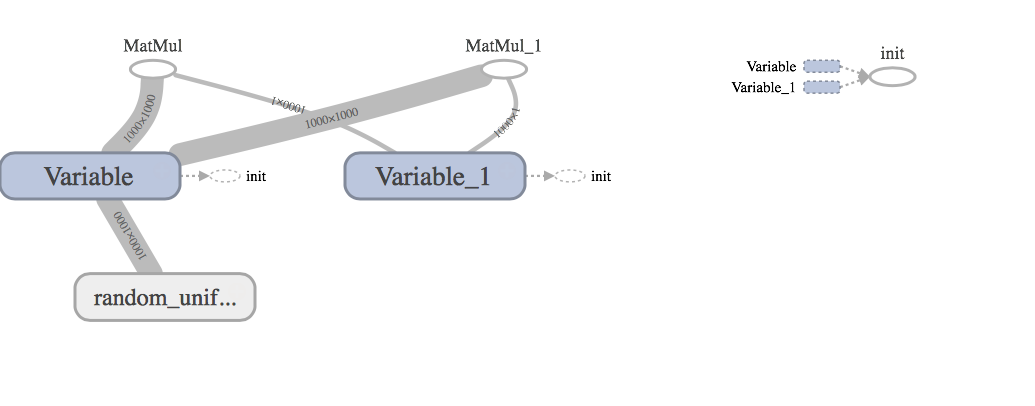
\includegraphics{graph3.png}

    \begin{Verbatim}[commandchars=\\\{\}]
{\color{incolor}In [{\color{incolor}24}]:} \PY{n}{sess}\PY{o}{.}\PY{n}{close}\PY{p}{(}\PY{p}{)}
         \PY{n}{tf}\PY{o}{.}\PY{n}{reset\PYZus{}default\PYZus{}graph}\PY{p}{(}\PY{p}{)}
\end{Verbatim}


    \hypertarget{numpy-style-slicing-is-not-supported}{%
\subsection{Numpy Style Slicing is Not
Supported!}\label{numpy-style-slicing-is-not-supported}}

Slicing a matrix requires reshaping into a vector and using an index
vector.

\hypertarget{lets-look-at-linear-regression-in-tensorflow}{%
\subsection{Let's Look at Linear Regression in
TensorFlow}\label{lets-look-at-linear-regression-in-tensorflow}}

For another example, see
http://tneal.org/post/tensorflow-iris/TensorFlowIris/.

    \begin{Verbatim}[commandchars=\\\{\}]
{\color{incolor}In [{\color{incolor}25}]:} \PY{n}{w}\PY{o}{=}\PY{n}{tf}\PY{o}{.}\PY{n}{Variable}\PY{p}{(}\PY{n}{tf}\PY{o}{.}\PY{n}{random\PYZus{}uniform}\PY{p}{(}\PY{p}{[}\PY{l+m+mi}{4}\PY{p}{,} \PY{l+m+mi}{1}\PY{p}{]}\PY{p}{)}\PY{p}{)}
\end{Verbatim}


    \begin{Verbatim}[commandchars=\\\{\}]
{\color{incolor}In [{\color{incolor}26}]:} \PY{n}{sess} \PY{o}{=} \PY{n}{tf}\PY{o}{.}\PY{n}{Session}\PY{p}{(}\PY{p}{)}
\end{Verbatim}


    \begin{Verbatim}[commandchars=\\\{\}]
{\color{incolor}In [{\color{incolor}27}]:} \PY{n}{sess}\PY{o}{.}\PY{n}{run}\PY{p}{(}\PY{n}{w}\PY{p}{)}
\end{Verbatim}


    \begin{Verbatim}[commandchars=\\\{\}]

        ---------------------------------------------------------------------------

        FailedPreconditionError                   Traceback (most recent call last)

        /Applications/anaconda/lib/python3.5/site-packages/tensorflow/python/client/session.py in \_do\_call(self, fn, *args)
       1021     try:
    -> 1022       return fn(*args)
       1023     except errors.OpError as e:


        /Applications/anaconda/lib/python3.5/site-packages/tensorflow/python/client/session.py in \_run\_fn(session, feed\_dict, fetch\_list, target\_list, options, run\_metadata)
       1003                                  feed\_dict, fetch\_list, target\_list,
    -> 1004                                  status, run\_metadata)
       1005 


        /Applications/anaconda/lib/python3.5/contextlib.py in \_\_exit\_\_(self, type, value, traceback)
         65             try:
    ---> 66                 next(self.gen)
         67             except StopIteration:


        /Applications/anaconda/lib/python3.5/site-packages/tensorflow/python/framework/errors\_impl.py in raise\_exception\_on\_not\_ok\_status()
        465           compat.as\_text(pywrap\_tensorflow.TF\_Message(status)),
    --> 466           pywrap\_tensorflow.TF\_GetCode(status))
        467   finally:


        FailedPreconditionError: Attempting to use uninitialized value Variable
    	 [[Node: \_send\_Variable\_0 = \_Send[T=DT\_FLOAT, client\_terminated=true, recv\_device="/job:localhost/replica:0/task:0/cpu:0", send\_device="/job:localhost/replica:0/task:0/cpu:0", send\_device\_incarnation=545785210948208991, tensor\_name="Variable:0", \_device="/job:localhost/replica:0/task:0/cpu:0"](Variable)]]

        
    During handling of the above exception, another exception occurred:


        FailedPreconditionError                   Traceback (most recent call last)

        <ipython-input-27-e7d66903f6cd> in <module>()
    ----> 1 sess.run(w)
    

        /Applications/anaconda/lib/python3.5/site-packages/tensorflow/python/client/session.py in run(self, fetches, feed\_dict, options, run\_metadata)
        765     try:
        766       result = self.\_run(None, fetches, feed\_dict, options\_ptr,
    --> 767                          run\_metadata\_ptr)
        768       if run\_metadata:
        769         proto\_data = tf\_session.TF\_GetBuffer(run\_metadata\_ptr)


        /Applications/anaconda/lib/python3.5/site-packages/tensorflow/python/client/session.py in \_run(self, handle, fetches, feed\_dict, options, run\_metadata)
        963     if final\_fetches or final\_targets:
        964       results = self.\_do\_run(handle, final\_targets, final\_fetches,
    --> 965                              feed\_dict\_string, options, run\_metadata)
        966     else:
        967       results = []


        /Applications/anaconda/lib/python3.5/site-packages/tensorflow/python/client/session.py in \_do\_run(self, handle, target\_list, fetch\_list, feed\_dict, options, run\_metadata)
       1013     if handle is None:
       1014       return self.\_do\_call(\_run\_fn, self.\_session, feed\_dict, fetch\_list,
    -> 1015                            target\_list, options, run\_metadata)
       1016     else:
       1017       return self.\_do\_call(\_prun\_fn, self.\_session, handle, feed\_dict,


        /Applications/anaconda/lib/python3.5/site-packages/tensorflow/python/client/session.py in \_do\_call(self, fn, *args)
       1033         except KeyError:
       1034           pass
    -> 1035       raise type(e)(node\_def, op, message)
       1036 
       1037   def \_extend\_graph(self):


        FailedPreconditionError: Attempting to use uninitialized value Variable
    	 [[Node: \_send\_Variable\_0 = \_Send[T=DT\_FLOAT, client\_terminated=true, recv\_device="/job:localhost/replica:0/task:0/cpu:0", send\_device="/job:localhost/replica:0/task:0/cpu:0", send\_device\_incarnation=545785210948208991, tensor\_name="Variable:0", \_device="/job:localhost/replica:0/task:0/cpu:0"](Variable)]]

    \end{Verbatim}

    \begin{Verbatim}[commandchars=\\\{\}]
{\color{incolor}In [{\color{incolor}28}]:} \PY{n}{sess}\PY{o}{.}\PY{n}{run}\PY{p}{(}\PY{n}{tf}\PY{o}{.}\PY{n}{global\PYZus{}variables\PYZus{}initializer}\PY{p}{(}\PY{p}{)}\PY{p}{)}
\end{Verbatim}


    \begin{Verbatim}[commandchars=\\\{\}]
{\color{incolor}In [{\color{incolor}29}]:} \PY{n}{sess}\PY{o}{.}\PY{n}{run}\PY{p}{(}\PY{n}{w}\PY{p}{)}
\end{Verbatim}


\begin{Verbatim}[commandchars=\\\{\}]
{\color{outcolor}Out[{\color{outcolor}29}]:} array([[ 0.21173167],
                [ 0.71594012],
                [ 0.55553162],
                [ 0.00845778]], dtype=float32)
\end{Verbatim}
            
    \begin{Verbatim}[commandchars=\\\{\}]
{\color{incolor}In [{\color{incolor}30}]:} \PY{k}{def} \PY{n+nf}{f}\PY{p}{(}\PY{n}{X}\PY{p}{)}\PY{p}{:}
         	\PY{k}{return} \PY{n}{tf}\PY{o}{.}\PY{n}{matmul}\PY{p}{(}\PY{n}{X}\PY{p}{,} \PY{n}{w}\PY{p}{)}
\end{Verbatim}


    \begin{Verbatim}[commandchars=\\\{\}]
{\color{incolor}In [{\color{incolor}31}]:} \PY{k}{def} \PY{n+nf}{objective}\PY{p}{(}\PY{n}{X}\PY{p}{,} \PY{n}{Y}\PY{p}{)}\PY{p}{:}
         	\PY{k}{return} \PY{n}{tf}\PY{o}{.}\PY{n}{reduce\PYZus{}sum}\PY{p}{(}\PY{n}{tf}\PY{o}{.}\PY{n}{square}\PY{p}{(}\PY{n}{tf}\PY{o}{.}\PY{n}{subtract}\PY{p}{(}\PY{n}{Y}\PY{p}{,}\PY{n}{f}\PY{p}{(}\PY{n}{X}\PY{p}{)}\PY{p}{)}\PY{p}{)}\PY{p}{)}
\end{Verbatim}


    Let's generate some synthetic data, and see how we can get a numpy array
into TensorFlow.

    \begin{Verbatim}[commandchars=\\\{\}]
{\color{incolor}In [{\color{incolor}32}]:} \PY{n}{a} \PY{o}{=} \PY{n}{np}\PY{o}{.}\PY{n}{array}\PY{p}{(}\PY{p}{[}\PY{p}{[}\PY{l+m+mi}{1}\PY{p}{,} \PY{l+m+mi}{2}\PY{p}{,} \PY{l+m+mi}{3}\PY{p}{,} \PY{l+m+mi}{4}\PY{p}{]}\PY{p}{]}\PY{p}{,} \PY{n}{dtype}\PY{o}{=}\PY{n}{np}\PY{o}{.}\PY{n}{float32}\PY{p}{)}
         \PY{n}{a}
\end{Verbatim}


\begin{Verbatim}[commandchars=\\\{\}]
{\color{outcolor}Out[{\color{outcolor}32}]:} array([[ 1.,  2.,  3.,  4.]], dtype=float32)
\end{Verbatim}
            
    \begin{Verbatim}[commandchars=\\\{\}]
{\color{incolor}In [{\color{incolor}33}]:} \PY{n}{XX} \PY{o}{=} \PY{n}{np}\PY{o}{.}\PY{n}{random}\PY{o}{.}\PY{n}{rand}\PY{p}{(}\PY{l+m+mi}{10000}\PY{p}{,} \PY{l+m+mi}{4}\PY{p}{)}
         \PY{n}{XX}
\end{Verbatim}


\begin{Verbatim}[commandchars=\\\{\}]
{\color{outcolor}Out[{\color{outcolor}33}]:} array([[ 0.2978405 ,  0.51167069,  0.21030663,  0.8166861 ],
                [ 0.8610743 ,  0.73845028,  0.86269288,  0.43507281],
                [ 0.0254931 ,  0.59831671,  0.81338779,  0.29694047],
                {\ldots}, 
                [ 0.56366656,  0.39858554,  0.45267797,  0.89401097],
                [ 0.56901679,  0.5466776 ,  0.70618478,  0.59461648],
                [ 0.34110282,  0.86880576,  0.45805236,  0.75228494]])
\end{Verbatim}
            
    \begin{Verbatim}[commandchars=\\\{\}]
{\color{incolor}In [{\color{incolor}34}]:} \PY{n}{YY} \PY{o}{=} \PY{n}{np}\PY{o}{.}\PY{n}{dot}\PY{p}{(}\PY{n}{XX}\PY{p}{,} \PY{n}{a}\PY{o}{.}\PY{n}{transpose}\PY{p}{(}\PY{p}{)}\PY{p}{)}
         \PY{n}{YY}
\end{Verbatim}


\begin{Verbatim}[commandchars=\\\{\}]
{\color{outcolor}Out[{\color{outcolor}34}]:} array([[ 5.21884618],
                [ 6.66634475],
                [ 4.8500518 ],
                {\ldots}, 
                [ 6.2949154 ],
                [ 6.15939224],
                [ 6.46201116]])
\end{Verbatim}
            
    \begin{Verbatim}[commandchars=\\\{\}]
{\color{incolor}In [{\color{incolor}35}]:} \PY{n}{X} \PY{o}{=} \PY{n}{tf}\PY{o}{.}\PY{n}{placeholder}\PY{p}{(}\PY{n}{tf}\PY{o}{.}\PY{n}{float32}\PY{p}{,} \PY{p}{[}\PY{k+kc}{None}\PY{p}{,} \PY{l+m+mi}{4}\PY{p}{]}\PY{p}{)}
         \PY{n}{Y} \PY{o}{=} \PY{n}{tf}\PY{o}{.}\PY{n}{placeholder}\PY{p}{(}\PY{n}{tf}\PY{o}{.}\PY{n}{float32}\PY{p}{,} \PY{p}{[}\PY{k+kc}{None}\PY{p}{,} \PY{l+m+mi}{1}\PY{p}{]}\PY{p}{)}
\end{Verbatim}


    \textbf{Automatic differentiation} at work here - no more calculus by
hand.

    \begin{Verbatim}[commandchars=\\\{\}]
{\color{incolor}In [{\color{incolor}36}]:} \PY{n}{grad} \PY{o}{=} \PY{n}{tf}\PY{o}{.}\PY{n}{gradients}\PY{p}{(}\PY{n}{objective}\PY{p}{(}\PY{n}{X}\PY{p}{,}\PY{n}{Y}\PY{p}{)}\PY{p}{,} \PY{p}{[}\PY{n}{w}\PY{p}{]}\PY{p}{)}
\end{Verbatim}


    Let's set up the optimization problem. We want to adjust the weights
\texttt{w} in order to mimimize the sum of squared differences.

\begin{Shaded}
\begin{Highlighting}[]
\KeywordTok{def}\NormalTok{ objective(X, Y):}
    \ControlFlowTok{return}\NormalTok{ tf.reduce_sum(tf.square(tf.subtract(Y,f(X))))}
\end{Highlighting}
\end{Shaded}

    \begin{Verbatim}[commandchars=\\\{\}]
{\color{incolor}In [{\color{incolor}37}]:} \PY{n}{step} \PY{o}{=} \PY{n}{tf}\PY{o}{.}\PY{n}{constant}\PY{p}{(}\PY{l+m+mf}{1e\PYZhy{}5}\PY{p}{)}
\end{Verbatim}


    \begin{Verbatim}[commandchars=\\\{\}]
{\color{incolor}In [{\color{incolor}38}]:} \PY{n}{sess}\PY{o}{.}\PY{n}{run}\PY{p}{(}\PY{n}{tf}\PY{o}{.}\PY{n}{global\PYZus{}variables\PYZus{}initializer}\PY{p}{(}\PY{p}{)}\PY{p}{)}
\end{Verbatim}


    \begin{Verbatim}[commandchars=\\\{\}]
{\color{incolor}In [{\color{incolor}39}]:} \PY{k}{for} \PY{n}{i} \PY{o+ow}{in} \PY{n+nb}{range}\PY{p}{(}\PY{l+m+mi}{200}\PY{p}{)}\PY{p}{:}
         	\PY{n}{sess}\PY{o}{.}\PY{n}{run}\PY{p}{(}\PY{n}{tf}\PY{o}{.}\PY{n}{assign\PYZus{}add}\PY{p}{(}\PY{n}{w}\PY{p}{,} \PY{n}{tf}\PY{o}{.}\PY{n}{multiply}\PY{p}{(}\PY{o}{\PYZhy{}}\PY{n}{step}\PY{p}{,} \PY{n}{grad}\PY{p}{[}\PY{l+m+mi}{0}\PY{p}{]}\PY{p}{)}\PY{p}{)}\PY{p}{,} \PY{n}{feed\PYZus{}dict}\PY{o}{=}\PY{p}{\PYZob{}}\PY{n}{X}\PY{p}{:}\PY{n}{XX}\PY{p}{,} \PY{n}{Y}\PY{p}{:}\PY{n}{YY}\PY{p}{\PYZcb{}}\PY{p}{)}
\end{Verbatim}


    \begin{Verbatim}[commandchars=\\\{\}]
{\color{incolor}In [{\color{incolor}40}]:} \PY{n}{sess}\PY{o}{.}\PY{n}{run}\PY{p}{(}\PY{n}{w}\PY{p}{)}
\end{Verbatim}


\begin{Verbatim}[commandchars=\\\{\}]
{\color{outcolor}Out[{\color{outcolor}40}]:} array([[ 1.05474031],
                [ 2.00871181],
                [ 2.98940301],
                [ 3.94768739]], dtype=float32)
\end{Verbatim}
            
    What is \texttt{w}? Remember, we're trying to find the weights that fit

\begin{Shaded}
\begin{Highlighting}[]
\KeywordTok{def}\NormalTok{ f(X):}
    \ControlFlowTok{return}\NormalTok{ tf.matmul(X, w)}
\end{Highlighting}
\end{Shaded}

to \texttt{Y}.

    \begin{Verbatim}[commandchars=\\\{\}]
{\color{incolor}In [{\color{incolor}41}]:} \PY{n}{sess}\PY{o}{.}\PY{n}{run}\PY{p}{(}\PY{n}{objective}\PY{p}{(}\PY{n}{X}\PY{p}{,} \PY{n}{Y}\PY{p}{)}\PY{p}{)}
\end{Verbatim}


    \begin{Verbatim}[commandchars=\\\{\}]

        ---------------------------------------------------------------------------

        InvalidArgumentError                      Traceback (most recent call last)

        /Applications/anaconda/lib/python3.5/site-packages/tensorflow/python/client/session.py in \_do\_call(self, fn, *args)
       1021     try:
    -> 1022       return fn(*args)
       1023     except errors.OpError as e:


        /Applications/anaconda/lib/python3.5/site-packages/tensorflow/python/client/session.py in \_run\_fn(session, feed\_dict, fetch\_list, target\_list, options, run\_metadata)
       1003                                  feed\_dict, fetch\_list, target\_list,
    -> 1004                                  status, run\_metadata)
       1005 


        /Applications/anaconda/lib/python3.5/contextlib.py in \_\_exit\_\_(self, type, value, traceback)
         65             try:
    ---> 66                 next(self.gen)
         67             except StopIteration:


        /Applications/anaconda/lib/python3.5/site-packages/tensorflow/python/framework/errors\_impl.py in raise\_exception\_on\_not\_ok\_status()
        465           compat.as\_text(pywrap\_tensorflow.TF\_Message(status)),
    --> 466           pywrap\_tensorflow.TF\_GetCode(status))
        467   finally:


        InvalidArgumentError: You must feed a value for placeholder tensor 'Placeholder' with dtype float
    	 [[Node: Placeholder = Placeholder[dtype=DT\_FLOAT, shape=[], \_device="/job:localhost/replica:0/task:0/cpu:0"]()]]

        
    During handling of the above exception, another exception occurred:


        InvalidArgumentError                      Traceback (most recent call last)

        <ipython-input-41-3ccd8f6bf29a> in <module>()
    ----> 1 sess.run(objective(X, Y))
    

        /Applications/anaconda/lib/python3.5/site-packages/tensorflow/python/client/session.py in run(self, fetches, feed\_dict, options, run\_metadata)
        765     try:
        766       result = self.\_run(None, fetches, feed\_dict, options\_ptr,
    --> 767                          run\_metadata\_ptr)
        768       if run\_metadata:
        769         proto\_data = tf\_session.TF\_GetBuffer(run\_metadata\_ptr)


        /Applications/anaconda/lib/python3.5/site-packages/tensorflow/python/client/session.py in \_run(self, handle, fetches, feed\_dict, options, run\_metadata)
        963     if final\_fetches or final\_targets:
        964       results = self.\_do\_run(handle, final\_targets, final\_fetches,
    --> 965                              feed\_dict\_string, options, run\_metadata)
        966     else:
        967       results = []


        /Applications/anaconda/lib/python3.5/site-packages/tensorflow/python/client/session.py in \_do\_run(self, handle, target\_list, fetch\_list, feed\_dict, options, run\_metadata)
       1013     if handle is None:
       1014       return self.\_do\_call(\_run\_fn, self.\_session, feed\_dict, fetch\_list,
    -> 1015                            target\_list, options, run\_metadata)
       1016     else:
       1017       return self.\_do\_call(\_prun\_fn, self.\_session, handle, feed\_dict,


        /Applications/anaconda/lib/python3.5/site-packages/tensorflow/python/client/session.py in \_do\_call(self, fn, *args)
       1033         except KeyError:
       1034           pass
    -> 1035       raise type(e)(node\_def, op, message)
       1036 
       1037   def \_extend\_graph(self):


        InvalidArgumentError: You must feed a value for placeholder tensor 'Placeholder' with dtype float
    	 [[Node: Placeholder = Placeholder[dtype=DT\_FLOAT, shape=[], \_device="/job:localhost/replica:0/task:0/cpu:0"]()]]
    
    Caused by op 'Placeholder', defined at:
      File "/Applications/anaconda/lib/python3.5/runpy.py", line 193, in \_run\_module\_as\_main
        "\_\_main\_\_", mod\_spec)
      File "/Applications/anaconda/lib/python3.5/runpy.py", line 85, in \_run\_code
        exec(code, run\_globals)
      File "/Applications/anaconda/lib/python3.5/site-packages/ipykernel/\_\_main\_\_.py", line 3, in <module>
        app.launch\_new\_instance()
      File "/Applications/anaconda/lib/python3.5/site-packages/traitlets/config/application.py", line 658, in launch\_instance
        app.start()
      File "/Applications/anaconda/lib/python3.5/site-packages/ipykernel/kernelapp.py", line 474, in start
        ioloop.IOLoop.instance().start()
      File "/Applications/anaconda/lib/python3.5/site-packages/zmq/eventloop/ioloop.py", line 177, in start
        super(ZMQIOLoop, self).start()
      File "/Applications/anaconda/lib/python3.5/site-packages/tornado/ioloop.py", line 887, in start
        handler\_func(fd\_obj, events)
      File "/Applications/anaconda/lib/python3.5/site-packages/tornado/stack\_context.py", line 275, in null\_wrapper
        return fn(*args, **kwargs)
      File "/Applications/anaconda/lib/python3.5/site-packages/zmq/eventloop/zmqstream.py", line 440, in \_handle\_events
        self.\_handle\_recv()
      File "/Applications/anaconda/lib/python3.5/site-packages/zmq/eventloop/zmqstream.py", line 472, in \_handle\_recv
        self.\_run\_callback(callback, msg)
      File "/Applications/anaconda/lib/python3.5/site-packages/zmq/eventloop/zmqstream.py", line 414, in \_run\_callback
        callback(*args, **kwargs)
      File "/Applications/anaconda/lib/python3.5/site-packages/tornado/stack\_context.py", line 275, in null\_wrapper
        return fn(*args, **kwargs)
      File "/Applications/anaconda/lib/python3.5/site-packages/ipykernel/kernelbase.py", line 276, in dispatcher
        return self.dispatch\_shell(stream, msg)
      File "/Applications/anaconda/lib/python3.5/site-packages/ipykernel/kernelbase.py", line 228, in dispatch\_shell
        handler(stream, idents, msg)
      File "/Applications/anaconda/lib/python3.5/site-packages/ipykernel/kernelbase.py", line 390, in execute\_request
        user\_expressions, allow\_stdin)
      File "/Applications/anaconda/lib/python3.5/site-packages/ipykernel/ipkernel.py", line 196, in do\_execute
        res = shell.run\_cell(code, store\_history=store\_history, silent=silent)
      File "/Applications/anaconda/lib/python3.5/site-packages/ipykernel/zmqshell.py", line 501, in run\_cell
        return super(ZMQInteractiveShell, self).run\_cell(*args, **kwargs)
      File "/Applications/anaconda/lib/python3.5/site-packages/IPython/core/interactiveshell.py", line 2717, in run\_cell
        interactivity=interactivity, compiler=compiler, result=result)
      File "/Applications/anaconda/lib/python3.5/site-packages/IPython/core/interactiveshell.py", line 2821, in run\_ast\_nodes
        if self.run\_code(code, result):
      File "/Applications/anaconda/lib/python3.5/site-packages/IPython/core/interactiveshell.py", line 2881, in run\_code
        exec(code\_obj, self.user\_global\_ns, self.user\_ns)
      File "<ipython-input-35-bfdb0d5263c1>", line 1, in <module>
        X = tf.placeholder(tf.float32, [None, 4])
      File "/Applications/anaconda/lib/python3.5/site-packages/tensorflow/python/ops/array\_ops.py", line 1502, in placeholder
        name=name)
      File "/Applications/anaconda/lib/python3.5/site-packages/tensorflow/python/ops/gen\_array\_ops.py", line 2149, in \_placeholder
        name=name)
      File "/Applications/anaconda/lib/python3.5/site-packages/tensorflow/python/framework/op\_def\_library.py", line 763, in apply\_op
        op\_def=op\_def)
      File "/Applications/anaconda/lib/python3.5/site-packages/tensorflow/python/framework/ops.py", line 2327, in create\_op
        original\_op=self.\_default\_original\_op, op\_def=op\_def)
      File "/Applications/anaconda/lib/python3.5/site-packages/tensorflow/python/framework/ops.py", line 1226, in \_\_init\_\_
        self.\_traceback = \_extract\_stack()
    
    InvalidArgumentError (see above for traceback): You must feed a value for placeholder tensor 'Placeholder' with dtype float
    	 [[Node: Placeholder = Placeholder[dtype=DT\_FLOAT, shape=[], \_device="/job:localhost/replica:0/task:0/cpu:0"]()]]


    \end{Verbatim}

    How do we fix this? Remember, \texttt{X} and \texttt{Y} are
\emph{placeholders}, and we need to tell TensorFlow what they should be
using \texttt{feed\_dict}. See
http://stackoverflow.com/questions/33810990/how-to-feed-a-placeholder.

    \begin{Verbatim}[commandchars=\\\{\}]
{\color{incolor}In [{\color{incolor}42}]:} \PY{n}{sess}\PY{o}{.}\PY{n}{run}\PY{p}{(}\PY{n}{objective}\PY{p}{(}\PY{n}{X}\PY{p}{,} \PY{n}{Y}\PY{p}{)}\PY{p}{,} \PY{n}{feed\PYZus{}dict}\PY{o}{=}\PY{p}{\PYZob{}}\PY{n}{X}\PY{p}{:}\PY{n}{XX}\PY{p}{,} \PY{n}{Y}\PY{p}{:}\PY{n}{YY}\PY{p}{\PYZcb{}}\PY{p}{)}
\end{Verbatim}


\begin{Verbatim}[commandchars=\\\{\}]
{\color{outcolor}Out[{\color{outcolor}42}]:} 4.9653783
\end{Verbatim}
            
    \hypertarget{finis}{%
\section{Finis}\label{finis}}

We're finished with this tutorial.

You can practice by using TensorFlow to
\href{http://www.learndatasci.com/predicting-housing-prices-linear-regression-using-python-pandas-statsmodels/}{fit
a linear regression model to housing prices}.

And to facilitate your TensorFlow work on GPU, you can
\href{https://blog.keras.io/running-jupyter-notebooks-on-gpu-on-aws-a-starter-guide.html}{run
notebooks on AWS}.

\href{https://medium.com/@vamsiramakrishnan/setup-a-cloud-based-machine-learning-system-from-scratch-aws-ec2-g-2x2-9216449d558d}{Set
up an instance with TensorFlow and Jupyter notebooks}.

\hypertarget{added-april-6-2017-the-day-after-the-presentation}{%
\subsection{Added April 6, 2017, the day after the
presentation}\label{added-april-6-2017-the-day-after-the-presentation}}

\href{https://www.oreilly.com/learning/hello-tensorflow}{A valuable,
different look at TensorFlow}.

\href{https://www.oreilly.com/learning/how-to-build-a-robot-that-sees-with-100-and-tensorflow}{Building
a robot that sees with TensorFlow} - hardware meets TensorFlow.

\href{https://www.packtpub.com/books/content/training-neural-networks-efficiently-using-keras}{Training
Neural Networks with Keras} - compare to tutorials for neural networks
that use just TensorFlow.


    % Add a bibliography block to the postdoc
    
    
    
    \end{document}
